% =============================================================================
%  slides.tex (docs/presentation4): 15 minute overview of the RISC-V vector (RVV)
%  work in pystencils and waLBerla, for listeners who know software but not this
%  project. A copy of docs/presentation3 with a new benchmark: waLBerla's
%  lid-driven cavity (app SweepgenLdcCPU) instead of the periodic box, measured
%  with GCC and with Clang. Build with ./build.sh (output: build/slides.pdf).
%
%  Sources of every number: the presentation4 board session (scripts/presentation4/
%  all.sh, raw logs in docs/presentation4/board-logs/) and the progress log
%  docs/presentation4/presentation4-progress-opus5.5.md, which also holds the
%  verification results. Numbers that come from the periodic box of presentation3
%  (docs/manual/reports/r02, r03) are labelled as such on the slide.
%
%  Writing rules: plain English, short sentences, no em/en dashes as
%  punctuation, every name explained where it first appears and again in the
%  glossary at the end.
% =============================================================================
\documentclass[aspectratio=169,10pt,t]{beamer}

\usepackage[T1]{fontenc}
\usepackage[utf8]{inputenc}
\usepackage[sfdefault,lining]{FiraSans}
\usepackage[varqu]{inconsolata}
\usefonttheme{professionalfonts}
\usepackage{amsmath,amssymb}
\usepackage{booktabs,array,tabularx}
\usepackage{pifont}
\usepackage{appendixnumberbeamer}

\usepackage{tikz}
\usetikzlibrary{positioning,arrows.meta,calc,fit,backgrounds,decorations.pathreplacing,patterns}
\usepackage{pgfplots}
\usepackage{multimedia}   % the flow film: \movie links figures/cavity-movie/cavity.avi (played by pdfpc)
\pgfplotsset{compat=1.18}

% ---- Colours (the same as in docs/manual, so slides and reports match) --------
\definecolor{psblue}{HTML}{1F5FA8}
\definecolor{psteal}{HTML}{127A72}
\definecolor{psorange}{HTML}{C8641A}
\definecolor{psred}{HTML}{B3261E}
\definecolor{psgray}{HTML}{5F6368}
\definecolor{codebg}{HTML}{F6F8FA}
\definecolor{psviolet}{HTML}{7A3E9D}   % generated code (build-run figure)
\newif\ifbrmarkers                       % markers in figures/build-run.tex
%   Meaning of the colours in every figure:
%   teal = added and measured, orange = in the code but not measured yet,
%   red = tried and dropped (or: what was wrong before), blue = facts about the hardware.

% ---- Beamer look ------------------------------------------------------------------
\setbeamersize{text margin left=8mm,text margin right=8mm}
\setbeamertemplate{navigation symbols}{}
\setbeamercolor{normal text}{fg=black!88}
\setbeamercolor{structure}{fg=psblue}
\setbeamercolor{frametitle}{fg=psblue!80!black}
\setbeamerfont{frametitle}{size=\large,series=\bfseries}
\setbeamercolor{itemize item}{fg=psblue}
\setbeamercolor{itemize subitem}{fg=psgray}
\setbeamertemplate{itemize item}{\raisebox{0.15ex}{\small$\bullet$}}
\setbeamertemplate{itemize subitem}{\raisebox{0.1ex}{\scriptsize$\circ$}}
\setlength{\leftmargini}{1.1em}
\setlength{\leftmarginii}{1.1em}
\setbeamercolor{takeaway}{bg=psblue!8,fg=black!88}

\setbeamertemplate{frametitle}{%
  \nointerlineskip\vskip3mm
  \hbox to \textwidth{%
    \usebeamerfont{frametitle}\usebeamercolor[fg]{frametitle}\insertframetitle\hfil
    {\usebeamerfont{footline}\scriptsize\color{psgray}\insertsectionhead}}%
  \vskip1.5mm
  {\color{psblue!40}\hrule height 0.5pt}%
  \vskip1mm}

\setbeamertemplate{footline}{%
  \hbox to \paperwidth{\hspace*{8mm}{\color{psgray}\tiny RISC-V vectors in pystencils and waLBerla}%
    \hfil{\color{psgray}\tiny\insertframenumber\,/\,\inserttotalframenumber}\hspace*{8mm}}%
  \vskip2.5mm}

% ---- Macros -------------------------------------------------------------------------
\newcommand{\presenter}{Saleh}            % edit: name on the title slide
\newcommand{\sx}[1]{#1\ensuremath{\times}} % a speedup factor, e.g. \sx{5.24}
\newcommand{\term}[1]{\textcolor{psblue!85!black}{\textbf{#1}}} % a name, defined right here
\newcommand{\code}[1]{\texttt{#1}}
\newcommand{\yes}{\textcolor{psteal}{\ding{51}}}
\newcommand{\no}{\textcolor{psgray!70}{$\cdot$}}
\newcommand{\tagdot}[1]{\tikz[baseline=-0.6ex]\fill[#1] (0,0) circle (0.9mm);} % colour dot
%   \todo{text}: a measurement or fact that is still missing. Shown in red; build with
%   ./build.sh final to hide all of them (it defines \hidetodos). ./build.sh lists them.
\newif\ifshowtodos \showtodostrue
\ifdefined\hidetodos \showtodosfalse \fi
\newcommand{\todo}[1]{\ifshowtodos{\scriptsize\textcolor{psred}{\textbf{[TODO: #1]}}}\fi}
%   \takeaway{text}: the one sentence to remember, at the bottom of a slide
\newcommand{\takeaway}[1]{\par\vfill
  \begin{beamercolorbox}[wd=\textwidth,sep=4pt,rounded=true]{takeaway}
    \small #1
  \end{beamercolorbox}}

% ---- TikZ styles shared by the figures ------------------------------------------------
\tikzset{
  box/.style={draw=psgray!80,fill=white,rounded corners=2pt,align=center,
    font=\footnotesize,inner sep=3pt,minimum height=7mm},
  added/.style={box,fill=psteal!12,draw=psteal!90!black,line width=0.6pt},
  pending/.style={box,fill=psorange!12,draw=psorange!90!black,line width=0.6pt},
  wrong/.style={box,fill=psred!7,draw=psred!80!black,line width=0.6pt},
  info/.style={box,fill=psblue!7,draw=psblue!70!black},
  quiet/.style={box,fill=psgray!8,draw=psgray!60,text=psgray!90!black},
  arr/.style={-{Stealth[length=2mm]},semithick,draw=psgray!90!black},
  lbl/.style={font=\scriptsize,text=psgray!90!black,align=center},
  codebox/.style={box,fill=codebg,font=\ttfamily\scriptsize,align=left,inner sep=4pt},
}

% ---- pgfplots styles shared by the result figures ---------------------------------------
%   onecore: one core, x = 8 builds (figures/speedup-1core-<prec>.tex, figures/mlups-1core.tex)
%   clang1/clang1legend: Clang as a white diamond next to its bar, no number
%   mc + pl/bs/av/rv/sp/cl/cllegend: several cores, x = 1, 4, 8 cores
%     (figures/mlups-multicore.tex, figures/speedup-multicore-<prec>.tex); each figure sets ymax
\pgfplotsset{
  onecore/.style={
    width=\textwidth, ymin=0,
    symbolic x coords={plain,plainav,best,bestav,rvv,pf,aa,split},
    xtick={plain,plainav,best,bestav,rvv,pf,aa,split},
    xticklabels={{plain scalar},{plain scalar,\\auto-vectorized},{best scalar},
      {best scalar,\\auto-vectorized},{RVV,\\AB pattern},{RVV,\\+ prefetch},
      {RVV, + in place\\(AA pattern)},{\textbf{RVV, AA,}\\\textbf{split loop,}\\\textbf{no prefetch}}},
    xticklabel style={align=center,font=\scriptsize,anchor=north},
    tick label style={font=\scriptsize}, label style={font=\scriptsize},
    enlarge x limits=0.065,
    legend style={font=\scriptsize,draw=psgray!50},
    nodes near coords, point meta=explicit symbolic,
    ymajorgrids, grid style={psgray!20}},
  clang1/.style={sharp plot,only marks,mark=diamond*,mark size=2.4pt,
    mark options={fill=white,draw=black!85},nodes near coords={}},
  clang1legend/.style={legend image code/.code={\draw[mark=diamond*,mark size=2.4pt,
    mark options={fill=white,draw=black!85}] plot coordinates {(0.15cm,0cm)};}},
  mc/.style={
    ybar=1pt, bar width=5pt, width=6.9cm, height=4.7cm, ymin=0,
    symbolic x coords={1,4,8}, xtick=data,
    xticklabels={1 core,4 cores,8 cores},
    enlarge x limits=0.22,
    tick label style={font=\scriptsize}, label style={font=\scriptsize},
    title style={font=\small\bfseries,yshift=-1.5ex},
    ymajorgrids, grid style={psgray!20},
    nodes near coords, point meta=explicit symbolic,
    nodes near coords style={font=\tiny,rotate=90,anchor=west,inner xsep=4pt}},
  pl/.style={fill=psgray!30,draw=psgray,bar shift=-12pt},
  bs/.style={fill=psgray!75,draw=psgray!90!black,bar shift=-6pt},
  av/.style={pattern=north east lines,pattern color=psgray!90!black,draw=psgray!90!black,bar shift=0pt},
  rv/.style={fill=psteal!55,draw=psteal!80!black,bar shift=6pt},
  sp/.style={fill=psteal!90!black,draw=psteal!60!black,bar shift=12pt},
  cl/.style={sharp plot,only marks,mark=diamond*,mark size=1.8pt,
    mark options={fill=white,draw=black!85},nodes near coords={},forget plot},
  cllegend/.style={legend image code/.code={\draw[mark=diamond*,mark size=1.8pt,
    mark options={fill=white,draw=black!85}] plot coordinates {(0.12cm,0cm)};}},
}

\title{Vector instructions for a generated fluid simulation on RISC-V}
\subtitle{What we added to pystencils and waLBerla, how it works, and what it gives in a lid-driven cavity on the SpacemiT X60, with GCC and Clang}
\author{\presenter}
\date{November 2026}

\begin{document}

% =============================================================================
\begin{frame}[plain]
  \begin{tikzpicture}[remember picture,overlay]
    % a strip of 8 "vector lanes" along the top edge
    \foreach \k in {0,...,7}
      \fill[psblue!\the\numexpr 25+8*\k\relax] ([xshift=\k*20mm]current page.north west) rectangle ++(19.6mm,-3mm);
    \node[anchor=north west,text width=136mm,align=left,inner sep=0pt,
          execute at begin node={\hyphenpenalty=10000\exhyphenpenalty=10000}]
      at ([xshift=12mm,yshift=-22mm]current page.north west) {%
      {\LARGE\bfseries\color{psblue!80!black}\inserttitle\par}
      \vspace{5mm}
      {\large\color{black!75}\insertsubtitle\par}
      \vspace{14mm}
      {\normalsize\insertauthor\par}
      \vspace{1mm}
      {\normalsize\color{psgray}\insertdate\par}};
  \end{tikzpicture}
\end{frame}

% =============================================================================
% =============================================================================
\section{Background}

\begin{frame}{The benchmark: a lid-driven cavity}
  \vspace{1mm}
  \begin{columns}[T,onlytextwidth]
    \column{0.40\textwidth}
    \centering% Slide "The benchmark": the lid-driven cavity of waLBerla's UniformGridCPU LDC scenario, as the
% benchmark SweepgenLdcCPU sets it up (its README): a closed box, the top face (y max) moves with
% (0.05, 0, 0), the other five faces are fixed walls; the fluid starts at rest and the lid drags it
% into a rotating flow. Cross-section in the x-y plane, 2D sketch (the vortex is only indicative).
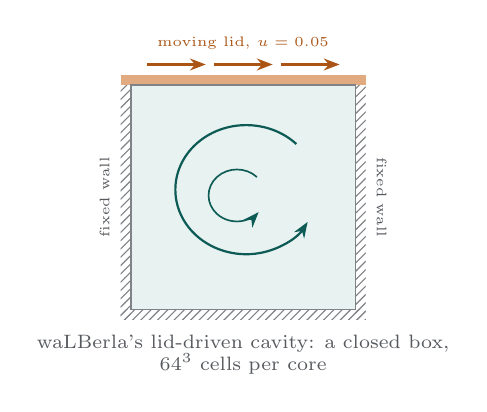
\begin{tikzpicture}
  \def\L{2.85}
  \def\t{0.13}
  % fluid
  \fill[psteal!10] (0,0) rectangle (\L,\L);
  % fixed walls (left, right, bottom): hatched
  \fill[pattern=north east lines,pattern color=psgray!80] (-\t,-\t) rectangle (0,\L);
  \fill[pattern=north east lines,pattern color=psgray!80] (\L,-\t) rectangle (\L+\t,\L);
  \fill[pattern=north east lines,pattern color=psgray!80] (-\t,-\t) rectangle (\L+\t,0);
  % the lid
  \fill[psorange!55] (-\t,\L) rectangle (\L+\t,\L+\t);
  \draw[psgray!80] (0,0) rectangle (\L,\L);
  \foreach \x in {0.2,1.05,1.9}
    \draw[arr,psorange!85!black,very thick] (\x,\L+0.26) -- ++(0.75,0);
  \node[font=\tiny,text=psorange!85!black,anchor=south] at (\L/2,\L+0.33) {moving lid, $u = 0.05$};
  % the rotating flow
  \draw[arr,psteal!75!black,thick] (2.1,2.1) arc[start angle=45,end angle=330,x radius=0.9,y radius=0.82];
  \draw[arr,psteal!75!black] (1.6,1.68) arc[start angle=45,end angle=320,x radius=0.36,y radius=0.33];
  \node[font=\tiny,text=psgray!90!black,rotate=90,anchor=south] at (-\t-0.02,\L/2) {fixed wall};
  \node[font=\tiny,text=psgray!90!black,rotate=-90,anchor=south] at (\L+\t+0.02,\L/2) {fixed wall};
  \node[lbl,anchor=north] at (\L/2,-0.2) {waLBerla's lid-driven cavity: a closed box,\\$64^3$ cells per core};
\end{tikzpicture}

    \column{0.57\textwidth}
    \centering\resizebox{!}{4.1cm}{% Slide 3: the two halves of an LBM time step, drawn in 2D (9 directions) for readability.
% The real model, D3Q19, is 3D with 19 directions.
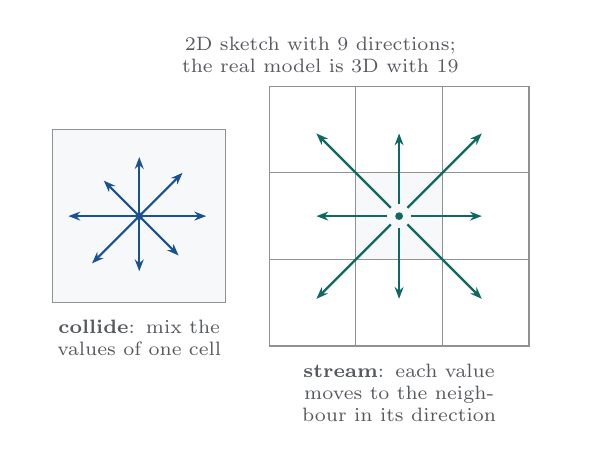
\begin{tikzpicture}[
    pdf/.style={-{Stealth[length=1.5mm]},thick,draw=psblue!85!black},
    mv/.style={-{Stealth[length=1.5mm]},thick,draw=psteal!85!black}]
  % ---- collide: one cell, one value per direction (arrow length = value)
  \draw[psgray!70,fill=codebg] (0,0.55) rectangle (2.2,2.75);
  \coordinate (c) at (1.1,1.65);
  \foreach \dx/\dy/\l in {1/0/0.85, 1/1/0.55, 0/1/0.75, -1/1/0.45, -1/0/0.9, -1/-1/0.6, 0/-1/0.7, 1/-1/0.5} {
    \draw[pdf] (c) -- ++({\dx*\l},{\dy*\l});
  }
  \fill[psblue!85!black] (c) circle (1.4pt);
  \node[lbl,anchor=north,text width=26mm] at (1.1,0.45) {\textbf{collide}: mix the values of one cell};

  % ---- stream: each value moves to the neighbour in its direction
  \begin{scope}[xshift=2.75cm]
    \foreach \i in {0,1,2} \foreach \j in {0,1,2}
      \draw[psgray!70,fill=white] (\i*1.1,\j*1.1) rectangle ++(1.1,1.1);
    \fill[codebg] (1.1,1.1) rectangle ++(1.1,1.1);
    \draw[psgray!70] (1.1,1.1) rectangle ++(1.1,1.1);
    \coordinate (s) at (1.65,1.65);
    \foreach \dx/\dy in {1/0, 1/1, 0/1, -1/1, -1/0, -1/-1, 0/-1, 1/-1}
      \draw[mv,shorten <=1.5mm] (s) -- ++({\dx*1.05},{\dy*1.05});
    \fill[psteal!85!black] (s) circle (1.4pt);
    \node[lbl,anchor=north,text width=33mm] at (1.65,-0.1) {\textbf{stream}: each value moves to the neighbour in its direction};
  \end{scope}
  \node[lbl,anchor=south,text width=60mm] at (3.4,3.35) {2D sketch with 9 directions; the real model is 3D with 19};
\end{tikzpicture}
}
  \end{columns}

  \vspace{1mm}
  {\small \term{waLBerla}: C++ fluid simulation framework. \term{Lattice Boltzmann method}, 19
  numbers per cell (\term{D3Q19}). Walls send back what flows into them (\term{bounce-back}).
  200 time steps; speed in \term{MLUP/s}, million cell updates per second.\par}
  \takeaway{Per cell and time step: 19 loads, about 200 operations, 19 stores. Walls: border cells only.}
\end{frame}

% -----------------------------------------------------------------------------
%  The two films (scripts/presentation4/laptop.sh part x86film, all.sh part movie + fetch_movie_board.sh):
%  the same program, SweepgenLdcCPU_explicit_cse_aa, f64, 64^3, warm-up 0, frame steps 16000 (k/40)^2, k = 0..40,
%  plus 210; each run from rest; middle plane drawn by scripts/presentation4/cavity_movie.py.
%  Laptop: generated with upstream pystencils 20d7dcf0 (build_x86.sh PYSTENCILS=upstream), x86 AVX intrinsics
%  (_mm256_*_pd), GCC 16.2.1 -O3 -march=native; the same kernel lines as with our fork, bit-identical fields
%  (field hash at 210, 1000, 4000 steps). Log board-logs/x86/cavity-movie.log.
%  Board: the verified all.sh executable (sha256 4cc7d6a9f3d1d81c), GCC 14.2.0, RVV; step 210 bit-identical to
%  all.sh (cavity_movie_board.sh check 2). Log board-logs/board/cavity-movie-board.log.
%  \movie only links the videos: build.sh copies them next to the PDF. Until the board film is fetched, its
%  slot shows a note (\IfFileExists), so the deck builds without it.
%  Agreement: scripts/presentation4/compare_movies.py (x86 log + slices against board log + slices), 42 frames:
%  worst relative energy difference 1.20e-14 (frame 41), worst middle-plane |du| / u_lid 5.07e-15; field hashes
%  equal only at step 0 (different instruction sets round differently). Board film: MOVIE PASS (step 210
%  bit-identical to all.sh), 47 copied files sha256-equal (fetch_movie_board.sh).
\begin{frame}{The flow we compute, on both machines}
  \vspace{1mm}
  \begin{columns}[T,onlytextwidth]
    \column{0.49\textwidth}
    \centering
    \movie[loop]{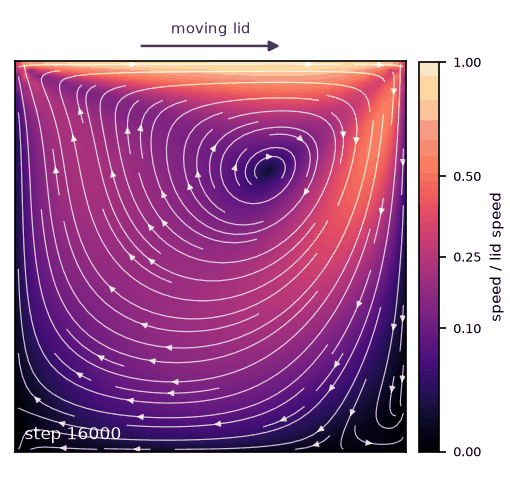
\includegraphics[height=4.3cm]{figures/cavity-movie/frame-41.png}}{figures/cavity-movie/cavity.avi}\par
    \vspace{1mm}
    {\scriptsize\textbf{Laptop}: Intel Core i9-13950HX, x86-64, AVX vectors (256 bits).\\
    pystencils' x86 code, not changed by us. GCC 16.2.\par}
    \column{0.49\textwidth}
    \centering
    \IfFileExists{figures/cavity-movie-board/frame-41.png}{%
      \movie[loop]{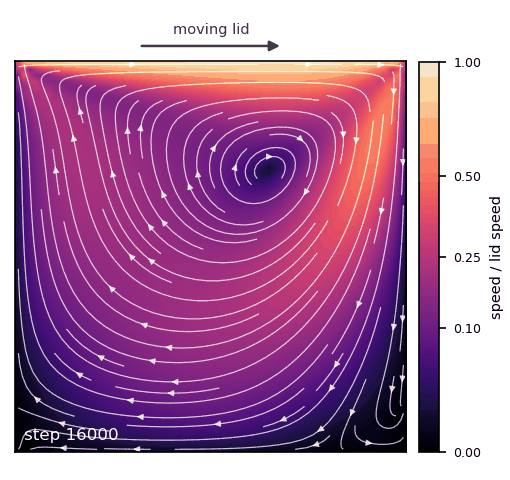
\includegraphics[height=4.3cm]{figures/cavity-movie-board/frame-41.png}}{figures/cavity-movie-board/cavity.avi}}{%
      {\setlength{\fboxsep}{0pt}\fbox{\parbox[c][4.3cm][c]{4.57cm}{\centering\scriptsize board film not fetched yet\\(\code{fetch\_movie\_board.sh})}}}}\par
    \vspace{1mm}
    {\scriptsize\textbf{Board}: SpacemiT X60, RISC-V, RVV 1.0 vectors (256 bits).\\
    Our pystencils RVV code. GCC 14.2.\par}
  \end{columns}
  \vspace{1.5mm}
  {\scriptsize\color{psgray}Same program: middle plane, colour = speed relative to the lid, lines = where the
  fluid goes; from rest to 16\,000 steps (a timed run: 210); f64, $64^3$ cells. In every frame the two agree to
  $1.2\cdot10^{-14}$ (energy) and $5\cdot10^{-15}$ of the lid speed. Click to play (\code{pdfpc}).\par}
  \takeaway{A real flow, and both machines compute the same one: they agree to 14 digits.}
\end{frame}

% -----------------------------------------------------------------------------
\begin{frame}{The hardware, and how the work is split}
  \vspace{3mm}
  \centering% Slide "The hardware, and how the work is split": the SpacemiT K1 on the Banana Pi BPI-F3
% (report r03, table "test system"): 8 X60 cores at 1.6 GHz in two clusters of 4; L1D 32 KiB per
% core, L2 512 KiB per cluster, no L3; 4 GB memory, about 357 cycles per DRAM miss (pointer chase,
% huge pages). The benchmark runs one MPI process with one 64^3 block per core.
% Right: one X60 core's 256-bit vector register as 8 f32 or 4 f64 lanes.
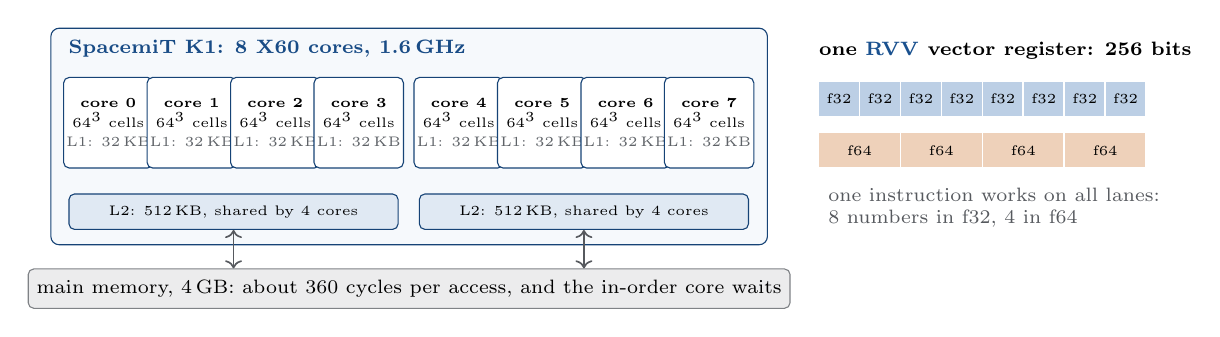
\begin{tikzpicture}[
    core/.style={box,minimum width=0.98cm,minimum height=1.15cm,fill=white,draw=psblue!70!black,
      font=\tiny,align=center,inner sep=1pt},
    l2/.style={box,fill=psblue!14,draw=psblue!70!black,font=\tiny,minimum height=4.5mm,inner sep=1pt},
    ln/.style={draw=white,line width=0.6pt,minimum height=4.5mm,inner sep=0pt,font=\tiny}]
  % ---- the chip -------------------------------------------------------------------
  \draw[psblue!70!black,fill=psblue!4,rounded corners=3pt] (0,0) rectangle (9.1,2.75);
  \node[anchor=north west,font=\scriptsize\bfseries,text=psblue!80!black] at (0.1,2.72)
    {SpacemiT K1: 8 X60 cores, 1.6\,GHz};
  \foreach \c/\xo in {0/0.2,1/4.65} {
    \foreach \k in {0,...,3} {
      \pgfmathtruncatemacro{\n}{4*\c+\k}
      \node[core] at (\xo+0.53+\k*1.06,1.55) {\textbf{core \n}\\[1pt]$64^3$ cells\\[1pt]{\color{psgray}L1: 32\,KB}};
    }
    \node[l2,minimum width=4.18cm] (l\c) at (\xo+2.12,0.42) {L2: 512\,KB, shared by 4 cores};
  }
  % ---- main memory -------------------------------------------------------------------
  \node[box,fill=psgray!12,minimum width=9.1cm,minimum height=5mm,font=\scriptsize,anchor=north]
    (mem) at (4.55,-0.3) {main memory, 4\,GB: about 360 cycles per access, and the in-order core waits};
  \foreach \c in {0,1} \draw[<->,semithick,psgray!90!black] (l\c.south) -- (l\c.south |- mem.north);

  % ---- one core's vector register --------------------------------------------------
  \begin{scope}[shift={(9.75,0.25)}]
    \def\w{0.52}
    \node[font=\scriptsize\bfseries,anchor=south west,inner sep=0pt] at (0,2.1) {one \term{RVV} vector register: 256 bits};
    \foreach \k in {0,...,7}
      \node[ln,fill=psblue!30,minimum width=\w cm] at (\k*\w+\w/2,1.6) {f32};
    \foreach \k in {0,...,3}
      \node[ln,fill=psorange!30,minimum width=2*\w cm] at (\k*2*\w+\w,0.95) {f64};
    \node[lbl,anchor=north west,align=left] at (0,0.6)
      {one instruction works on all lanes:\\8 numbers in f32, 4 in f64};
  \end{scope}
\end{tikzpicture}


  \vspace{4mm}
  \raggedright
  {\small One \term{MPI} process and one block per core. After every step, neighbouring blocks swap
  their border cells (\term{halo exchange}), and the wall pass updates the cells next to a wall.\par}
  \takeaway{One 256-bit operation per cycle: at best \sx{8} (f32) and \sx{4} (f64). These are our
    goals.}
\end{frame}

% -----------------------------------------------------------------------------
\begin{frame}{From source code to a running simulation}
  \vspace{1mm}
  \centering% From source to a running simulation (report r02, chapter "Code Generation" and its figure
% build-flow.tex). CMake configures; during "make", CMake runs the Python generator scripts
% (sweepgen sets jit = no_jit: generate only), then compiles the generated C++ together with
% the hand-written waLBerla core. The executable runs without Python. Everything ran on the
% board. Violet = generated code. Each column is one step; the small arrows between the
% headers carry the results from step to step (no wires across columns).
%
% With \brmarkerstrue (slide "Where each change lives") numbered markers show what we changed:
% blue = part 1, teal = part 2 (10 to 12: the last three changes, see the open-work slide).
% The markers sit on the nodes a2, g0, g2, g3, i1, i2 and cc.
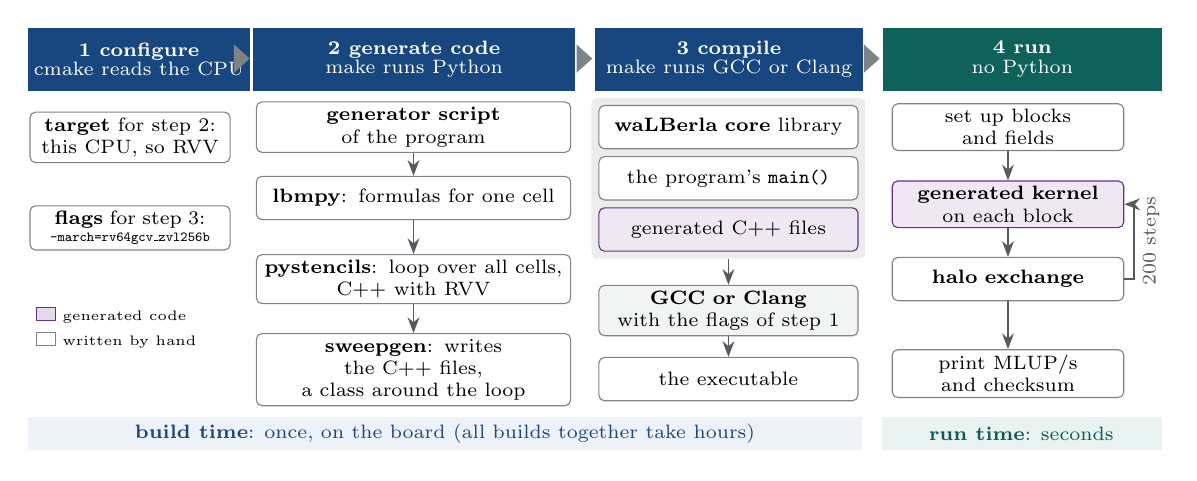
\begin{tikzpicture}[
    hdr/.style={font=\scriptsize\bfseries,text=white,align=center,inner sep=2pt,
      minimum height=8mm,anchor=north west},
    b/.style={box,font=\scriptsize,minimum height=5.5mm,inner sep=2pt,
      execute at begin node={\hyphenpenalty=10000\exhyphenpenalty=10000}},
    gen/.style={b,fill=psviolet!12,draw=psviolet!80!black},
    hdrarr/.style={fill=psgray!80},
    mk/.style={circle,text=white,font=\tiny\bfseries,inner sep=0pt,minimum size=3.7mm}]
  \ifbrmarkers\tikzset{mkl/.style={align=left}}\else\tikzset{mkl/.style={}}\fi
  % ---- column headers, with arrows from step to step --------------------------------
  \node[hdr,fill=psblue!75!black,minimum width=2.6cm] at (0,0)
    {1 configure\\[-1pt]{\mdseries cmake reads the CPU}};
  \node[hdr,fill=psblue!75!black,minimum width=4.1cm] at (2.85,0)
    {2 generate code\\[-1pt]{\mdseries make runs Python}};
  \node[hdr,fill=psblue!75!black,minimum width=3.4cm] at (7.2,0)
    {3 compile\\[-1pt]{\mdseries make runs GCC or Clang}};
  \node[hdr,fill=psteal!80!black,minimum width=3.55cm] at (10.85,0)
    {4 run\\[-1pt]{\mdseries no Python}};
  \foreach \x in {2.62,6.97,10.62}
    \fill[hdrarr] (\x,-0.22) -- ++(0.2,-0.18) -- ++(-0.2,-0.18) -- cycle;

  % ---- 1 configure: two settings for the later steps --------------------------------
  \node[b,text width=2.4cm] (a3) at (1.3,-1.4) {\textbf{target} for step 2:\\this CPU, so RVV};
  \node[b,text width=2.4cm,font=\tiny] (a2) at (1.3,-2.55)
    {{\scriptsize\textbf{flags} for step 3:}\\\code{-march=rv64gcv\_zvl256b}};
  \node[anchor=north west,font=\tiny,align=left,inner sep=0pt] at (0.1,-3.55)
    {\tikz\fill[psviolet!20,draw=psviolet!80!black] (0,0) rectangle (2.4mm,1.6mm);\ generated code\\[3pt]
     \tikz\draw[psgray!80] (0,0) rectangle (2.4mm,1.6mm);\ written by hand};

  % ---- 2 generate: the Python tool chain ---------------------------------------------
  \node[b,text width=3.85cm] (g0) at (4.9,-1.27) {\textbf{generator script} of the program};
  \node[b,text width=3.85cm] (g1) at (4.9,-2.17) {\textbf{lbmpy}: formulas for one cell};
  \node[b,text width=3.85cm] (g2) at (4.9,-3.2) {\textbf{pystencils}: loop over all cells,\\C++ with RVV};
  \node[b,text width=3.85cm] (g3) at (4.9,-4.35) {\textbf{sweepgen}: writes the C++ files,\\a class around the loop};
  \foreach \u/\v in {g0/g1,g1/g2,g2/g3} \draw[arr] (\u) -- (\v);

  % ---- 3 compile: hand-written and generated C++ together ----------------------------
  \node[b,mkl,text width=3.15cm] (i1) at (8.9,-1.27) {\textbf{waLBerla core} library};
  \node[b,mkl,text width=3.15cm] (i2) at (8.9,-1.92) {the program's \code{main()}};
  \node[gen,text width=3.15cm] (i0) at (8.9,-2.57) {generated C++ files};
  \begin{scope}[on background layer]
    \node[fill=psgray!12,rounded corners=2pt,inner sep=2.5pt,fit=(i1)(i2)(i0)] (src) {};
  \end{scope}
  \node[b,text width=3.15cm,fill=psgray!8] (cc) at (8.9,-3.6) {\textbf{GCC or Clang}\\with the flags of step 1};
  \node[b,text width=3.15cm] (exe) at (8.9,-4.47) {the executable};
  \draw[arr] (src) -- (cc);
  \draw[arr] (cc) -- (exe);

  % ---- 4 run: set up, then the time loop ---------------------------------------------
  \node[b,text width=2.8cm] (r0) at (12.45,-1.27) {set up blocks and fields};
  \node[gen,text width=2.8cm] (r1) at (12.45,-2.25) {\textbf{generated kernel}\\on each block};
  \node[b,text width=2.8cm] (r2) at (12.45,-3.2) {\textbf{halo exchange}};
  \node[b,text width=2.8cm] (r3) at (12.45,-4.4) {print MLUP/s and checksum};
  \draw[arr] (r0) -- (r1);
  \draw[arr] (r1) -- (r2);
  \draw[arr] (r2.east) -- ++(0.12,0) |- (r1.east);
  \node[lbl,rotate=90] at (14.27,-2.72) {200 steps};
  \draw[arr] (r2) -- (r3);

  % ---- time bands ----------------------------------------------------------------------
  \fill[psblue!8] (0,-4.95) rectangle (10.6,-5.37);
  \node[font=\scriptsize,text=psblue!75!black] at (5.3,-5.16)
    {\textbf{build time}: once, on the board (all builds together take hours)};
  \fill[psteal!10] (10.85,-4.95) rectangle (14.4,-5.37);
  \node[font=\scriptsize,text=psteal!75!black] at (12.62,-5.16) {\textbf{run time}: seconds};

  % ---- markers: what we changed ------------------------------------------------------
  \ifbrmarkers
    \tikzset{mk/.append style={minimum size=3.2mm}}
    %   \brmark: on top of the box's upper border; \brmarkin: inside the box, at its right end
    \def\brmark#1#2#3#4{% node, slot (0 = rightmost), colour, number
      \node[mk,fill=#3] at ([xshift={-2.2mm-#2*3.6mm},yshift=1.3mm]#1.north east) {#4};}
    \def\brmarkin#1#2#3#4{%
      \node[mk,fill=#3] at ([xshift={-2.2mm-#2*3.6mm}]#1.east) {#4};}
    \brmark{a2}{0}{psblue}{1}   \brmark{a2}{1}{psteal}{8}
    \brmark{g0}{0}{psblue}{3}
    \brmark{g2}{0}{psblue}{2}   \brmark{g2}{1}{psteal}{5}   \brmark{g2}{2}{psteal}{12}
    \brmark{g3}{0}{psteal}{6}   \brmark{g3}{1}{psteal}{10}
    \brmarkin{i1}{0}{psteal}{11} \brmarkin{i1}{1}{psteal}{7}
    \brmarkin{i2}{0}{psteal}{9}    \brmarkin{i2}{1}{psblue}{3}
    \brmark{cc}{0}{psblue}{4}
  \fi
\end{tikzpicture}

  \takeaway{Python only runs while the program is built. The program that runs is plain C++.}
\end{frame}

% =============================================================================
\section{Part 1: make it work}

\begin{frame}{What we added, and the builds we compare}
  \vspace{2mm}
  \centering% Slide "What we added": the four pieces that were missing on RISC-V (report r02, chapter "What
% Was Missing"): compiler flags in the waLBerla build, an RVV target in pystencils, a compile-time
% check for the register width, and a benchmark program that asks for vector code.
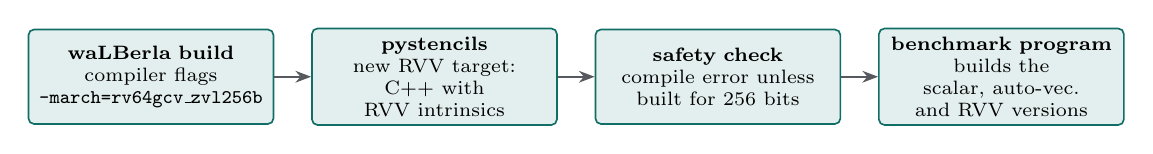
\begin{tikzpicture}[
    pc/.style={added,text width=29mm,minimum height=12mm,font=\scriptsize,align=center}]
  \def\dx{3.6}
  \node[pc] (a1) at (0,0)     {\textbf{waLBerla build}\\compiler flags\\\code{-march=rv64gcv\_zvl256b}};
  \node[pc] (a2) at (\dx,0)   {\textbf{pystencils}\\new RVV target:\\C++ with RVV intrinsics};
  \node[pc] (a3) at (2*\dx,0) {\textbf{safety check}\\compile error unless\\built for 256 bits};
  \node[pc] (a4) at (3*\dx,0) {\textbf{benchmark program}\\builds the scalar, auto-vec.\\and RVV versions};
  \foreach \u/\v in {a1/a2,a2/a3,a3/a4} \draw[arr] (\u) -- (\v);
\end{tikzpicture}


  \vspace{5mm}
  {\footnotesize\renewcommand{\arraystretch}{1.15}
  \begin{tabular}{@{}lll@{}}
    \toprule
    \textbf{build} & \textbf{kernel} & \textbf{compiler flags}\\
    \midrule
    plain scalar & plain C++ & \code{-march=rv64gc} for every file: no vector instruction\\
    auto-vectorized & plain C++ & \code{-march=rv64gcv\_zvl256b}: compiler may vectorize\\
    best scalar & plain C++ with \term{CSE} and in-place update & \code{-march=rv64gc} for every file\\
    \textbf{RVV} & \textbf{RVV intrinsics from pystencils} & \code{-march=rv64gcv\_zvl256b}\\
    \bottomrule
  \end{tabular}\par}

  \vspace{2mm}
  {\scriptsize\color{psgray}Every build twice: \term{GCC}~14.2 and \term{Clang}~18.1, \code{-O3}; Clang also
  gets \code{-mtune=spacemit-x60} (GCC does not accept it). Speedup: MLUP/s divided by that of the
  plain scalar build of the same compiler, same session. CSE: each repeated part of the formulas is
  computed once.\par}
  \takeaway{Users change nothing: ``optimise for this machine'' now gives RVV code, as it gives AVX
    code on x86.}
\end{frame}

% =============================================================================
\section{Part 2: make it fast}

%  What a stream is. Sources: the generated StreamCollide (19 prefetch_read + 23 prefetch_write, one
%  per array; see figures/stream-def.tex); the quote: M. Wittmann, T. Zeiser, G. Hager, G. Wellein,
%  "Modeling and analyzing performance for highly optimized propagation steps of the lattice Boltzmann
%  method on sparse lattices", arXiv:1410.0412 (2014/2015), section 4.3.
\begin{frame}{What a data stream is, and why our loop has 42}
  \begin{columns}[T,onlytextwidth]
    \column{0.55\textwidth}
    \vspace{1mm}
    \centering% Slide "What a data stream is": the memory one step of the inner loop touches (AB pattern, the
% generated StreamCollide kernel). Each of the 19 values of a cell has its own array (waLBerla's
% fzyx layout); pull streaming reads value i at the neighbour x - c_i (still consecutive addresses
% along x), the AB pattern writes a second set of 19 arrays, and the kernel writes rho and u
% (4 arrays): 19 + 19 + 4 = 42 sequences of consecutive addresses, all advancing together.
% Evidence: the generated StreamCollide of SweepgenLdcCPU_explicit_cse_pf (GCC f32, board) has
% exactly 19 prefetch_read and 23 prefetch_write calls in its loop, one per array it walks through.
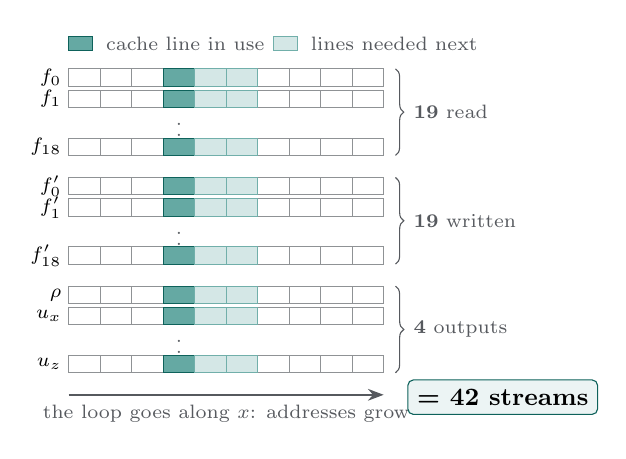
\begin{tikzpicture}[x=1cm,y=1cm]
  \tikzset{cl/.style={draw=psgray!70,fill=white,line width=0.3pt},
           clnow/.style={draw=psteal!80!black,fill=psteal!65,line width=0.3pt},
           clnext/.style={draw=psteal!60,fill=psteal!18,line width=0.3pt},
           arrlbl/.style={font=\scriptsize,anchor=east,inner sep=1pt}}
  %   \strip{y}{label}: one array as 10 cache lines; the loop is at line 3, lines 4 and 5 come next
  \newcommand{\strip}[2]{%
    \foreach \k in {0,...,9} \draw[cl] (\k*0.4,#1) rectangle ++(0.4,0.22);
    \draw[clnow] (1.2,#1) rectangle ++(0.4,0.22);
    \draw[clnext] (1.6,#1) rectangle ++(0.4,0.22);
    \draw[clnext] (2.0,#1) rectangle ++(0.4,0.22);
    \node[arrlbl] at (-0.05,#1+0.11) {#2};}
  \newcommand{\vdotsat}[1]{\node[font=\scriptsize,text=psgray] at (1.4,#1) {$\vdots$};}
  \newcommand{\grp}[4]{% y bottom, y top, count, what
    \draw[decorate,decoration={brace,amplitude=3pt},psgray!90!black] (4.15,#2) -- (4.15,#1)
      node[midway,right=3pt,font=\scriptsize,align=left] {\textbf{#3} #4};}

  \strip{3.5}{$f_0$} \strip{3.23}{$f_1$} \vdotsat{2.98} \strip{2.62}{$f_{18}$}
  \grp{2.62}{3.72}{19}{read}
  \strip{2.12}{$f'_0$} \strip{1.85}{$f'_1$} \vdotsat{1.6} \strip{1.24}{$f'_{18}$}
  \grp{1.24}{2.34}{19}{written}
  \strip{0.74}{$\rho$} \strip{0.47}{$u_x$} \vdotsat{0.22} \strip{-0.14}{$u_z$}
  \grp{-0.14}{0.96}{4}{outputs}

  \draw[arr] (0,-0.42) -- (4.0,-0.42) node[midway,below,lbl] {the loop goes along $x$: addresses grow};
  \node[draw=psteal!80!black,fill=psteal!8,rounded corners=2pt,font=\small\bfseries,anchor=west]
    at (4.3,-0.45) {= 42 streams};
  %   legend
  \draw[clnow] (0,3.95) rectangle ++(0.3,0.18);
  \node[lbl,anchor=west] at (0.35,4.04) {cache line in use};
  \draw[clnext] (2.6,3.95) rectangle ++(0.3,0.18);
  \node[lbl,anchor=west] at (2.95,4.04) {lines needed next};
\end{tikzpicture}

    \column{0.43\textwidth}
    \vspace{1mm}
    \begin{itemize}\small
      \item \term{Stream}: the loop reads or writes one array at consecutive addresses, cache line
            after cache line. The \term{hardware prefetcher} spots this and loads the next lines early.
      \item Each of the 19 values of a cell has its own array. One step of the loop reads 19 arrays,
            writes 19 others and 4 outputs ($\rho$, $u$): 42 streams.
      \item In place (AA): 23. A 7-point stencil: 6 (one array read in 5 rows, one written).
    \end{itemize}
  \end{columns}
  \vfill
  {\scriptsize\color{psgray}The term in lattice Boltzmann performance papers: ``concurrent memory streams
  (38 with OS-NT and 19 with AA)'' for D3Q19 (Wittmann et al., arXiv:1410.0412).\par}
  \takeaway{A stream is one sequence of addresses the loop walks through. Our loop walks through 42 at once.}
\end{frame}

% -----------------------------------------------------------------------------
%  Plot: figures/streams.tex (scripts/presentation4/streams_check.sh, streams-probe.log). Program numbers:
%  streams-ldc.log, python3 scripts/presentation4/streams_table.py docs/presentation4/board-logs/board:
%  GCC f32, 64^3, l2_miss per cell update (20 steps minus 0): explicit_cse 3.077, explicit_cse_aa 1.762,
%  explicit_cse_aa_split 0.341 (none of the three has software prefetch: 0 hint instructions);
%  stalled_cycle_backend 713.5 of 776 cycles per cell (1.6 GHz / 2.06 MLUP/s) for explicit_cse = 92 %.
\begin{frame}{The real limit: too many data streams}
  \begin{columns}[T,onlytextwidth]
    \column{0.52\textwidth}
    \centering% Slide 9: cost of concurrent read streams on one X60 core (r03, from board-logs/p2-stream-sweep.txt
% and p2-prefetch.txt): f32 vector loads, 4 MB per stream, huge pages.
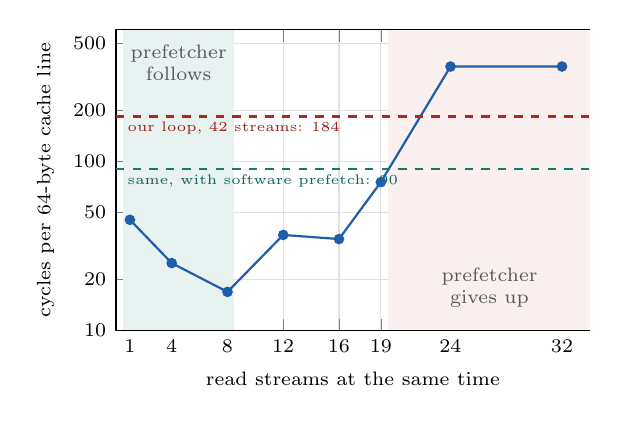
\begin{tikzpicture}
  \begin{semilogyaxis}[
      width=7.6cm, height=5.4cm,
      xlabel={read streams at the same time},
      ylabel={cycles per 64-byte cache line},
      xmin=0, xmax=34, ymin=10, ymax=600,
      xtick={1,4,8,12,16,19,24,32},
      ytick={10,20,50,100,200,500},
      yticklabels={10,20,50,100,200,500},
      grid=major, grid style={psgray!20},
      tick label style={font=\scriptsize}, label style={font=\scriptsize},
      every axis plot/.append style={thick},
    ]
    \fill[psteal!10] (axis cs:0.5,10) rectangle (axis cs:8.5,600);
    \node[lbl,anchor=north] at (axis cs:4.5,560) {prefetcher\\follows};
    \fill[psred!7] (axis cs:19.5,10) rectangle (axis cs:34,600);
    \node[lbl,anchor=south] at (axis cs:26.8,12) {prefetcher\\gives up};
    \addplot[color=psblue,mark=*,mark size=1.5pt] coordinates {
      (1,45.1) (4,25.0) (8,16.9) (12,36.7) (16,34.7) (19,75.3) (24,363.6) (32,363.7)};
    \draw[psred,thick,dashed] (axis cs:0,184.3) -- (axis cs:34,184.3);
    \node[font=\tiny,anchor=north west,text=psred!85!black,inner sep=1pt] at (axis cs:0.6,178)
      {our loop, 42 streams: 184};
    \draw[psteal,thick,dashed] (axis cs:0,90.4) -- (axis cs:34,90.4);
    \node[font=\tiny,anchor=north west,text=psteal!80!black,inner sep=1pt] at (axis cs:0.6,87)
      {same, with software prefetch: 90};
  \end{semilogyaxis}
\end{tikzpicture}

    \column{0.46\textwidth}
    \vspace{1mm}
    \begin{itemize}\small
      \item Plot: a test loop reading $R$ arrays, with the core's own counters (code on the next slides).
      \item Up to 19 streams the \term{hardware prefetchers} bring at least 4 of 5 lines in time. From 23
            on (with some offsets from 21), every line is late: it waits a full memory latency, about 360 cycles.
      \item Other array addresses do not move this cliff: it is the number of streams.
      \item Our program, same counter: 3.1 late lines per cell with 42 streams, 1.8 with 23 (in place),
            0.34 with the split loop.
    \end{itemize}
  \end{columns}
  \takeaway{The X60 follows about 20 streams, our loop has 42: the core waits for memory in 92\,\% of
    its cycles (42-stream build).}
\end{frame}

% -----------------------------------------------------------------------------
\begin{frame}{The stream test: the code behind the plot}
  \vspace{2mm}
  \centering% Slide "The stream test: the code behind the plot".
% Top: the timed loop of misc/x60-lab/probes/mem.cpp, function stream() (lines 124-158), simplified:
% the real code adds the 8 loads with a sum tree (a0+a1, a2+a3, ...) so they do not wait for each
% other, and has further options (touch-ahead loads, prefetch.w, cbo.zero, scalar loads) not used here.
% Each array is 4 MB (f32); the time is the best of 3 passes, read with the cycle counter
% (perf_event_open, probes/pmu.hpp). Built with g++ -O2 -march=rv64gcv_zvl256b_zicboz.
% Bottom: the commands and their results, all from presentation4's runs (scripts/presentation4/streams_check.sh):
% first three docs/presentation4/board-logs/board/streams-probe.log (tags a and c, reps=3), last two
% streams-pattern.log (best of 3 runs: 180.7 / 181.9 / 176.3 and 90.0 / 91.0 / 90.8; report 3 had 184.3 and 90.4).
% Printed by streams_table.py --tex; checked by check_figures.py.
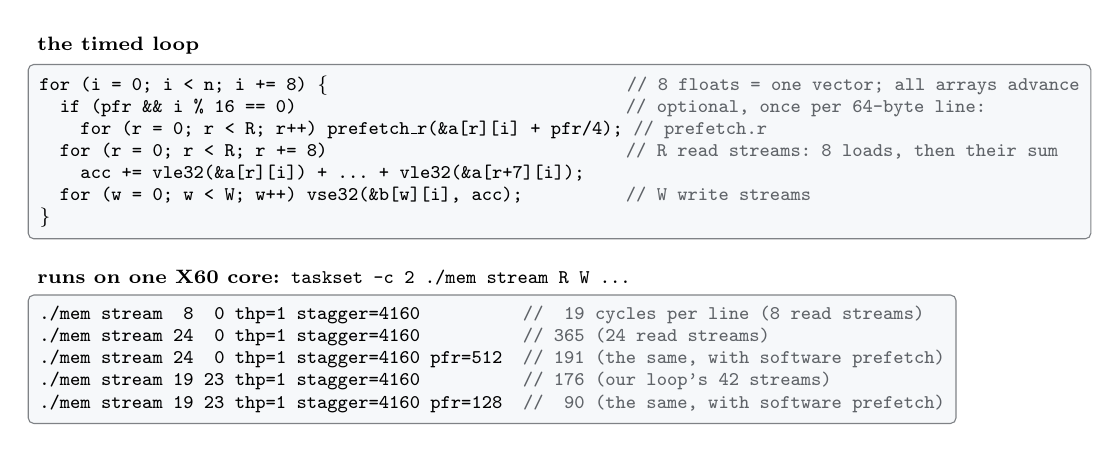
\begin{tikzpicture}
  \node[codebox,anchor=north west] (loop) at (0,0) {%
for\ (i\ =\ 0;\ i\ <\ n;\ i\ +=\ 8)\ \{\ \ \ \ \ \ \ \ \ \ \ \ \ \ \ \ \ \ \ \ \ \ \ \ \ \ \ \ \ \textcolor{psgray}{//\ 8\ floats\ =\ one\ vector;\ all\ arrays\ advance}\\
\ \ if\ (pfr\ \&\&\ i\ \%\ 16\ ==\ 0)\ \ \ \ \ \ \ \ \ \ \ \ \ \ \ \ \ \ \ \ \ \ \ \ \ \ \ \ \ \ \ \ \textcolor{psgray}{//\ optional,\ once\ per\ 64-byte\ line:}\\
\ \ \ \ for\ (r\ =\ 0;\ r\ <\ R;\ r++)\ prefetch\_r(\&a[r][i]\ +\ pfr/4);\ \textcolor{psgray}{//\ prefetch.r}\\
\ \ for\ (r\ =\ 0;\ r\ <\ R;\ r\ +=\ 8)\ \ \ \ \ \ \ \ \ \ \ \ \ \ \ \ \ \ \ \ \ \ \ \ \ \ \ \ \ \textcolor{psgray}{//\ R\ read\ streams:\ 8\ loads,\ then\ their\ sum}\\
\ \ \ \ acc\ +=\ vle32(\&a[r][i])\ +\ ...\ +\ vle32(\&a[r+7][i]);\\
\ \ for\ (w\ =\ 0;\ w\ <\ W;\ w++)\ vse32(\&b[w][i],\ acc);\ \ \ \ \ \ \ \ \ \ \textcolor{psgray}{//\ W\ write\ streams}\\
\}};
  \node[font=\scriptsize\bfseries,anchor=south west] at (loop.north west) {the timed loop};
  \node[codebox,anchor=north west] (cmd) at ([yshift=-7mm]loop.south west) {%
./mem\ stream\ \ 8\ \ 0\ thp=1\ stagger=4160\ \ \ \ \ \ \ \ \ \ \textcolor{psgray}{//\ \ 19\ cycles\ per\ line\ (8\ read\ streams)}\\
./mem\ stream\ 24\ \ 0\ thp=1\ stagger=4160\ \ \ \ \ \ \ \ \ \ \textcolor{psgray}{//\ 365\ (24\ read\ streams)}\\
./mem\ stream\ 24\ \ 0\ thp=1\ stagger=4160\ pfr=512\ \ \textcolor{psgray}{//\ 191\ (the\ same,\ with\ software\ prefetch)}\\
./mem\ stream\ 19\ 23\ thp=1\ stagger=4160\ \ \ \ \ \ \ \ \ \ \textcolor{psgray}{//\ 176\ (our\ loop's\ 42\ streams)}\\
./mem\ stream\ 19\ 23\ thp=1\ stagger=4160\ pfr=128\ \ \textcolor{psgray}{//\ \ 90\ (the\ same,\ with\ software\ prefetch)}};
  \node[font=\scriptsize\bfseries,anchor=south west] at (cmd.north west) {runs on one X60 core: \code{taskset -c 2 ./mem stream R W ...}};
\end{tikzpicture}


  \vspace{2mm}
  {\scriptsize\color{psgray}Simplified from \code{misc/x60-lab/probes/mem.cpp} (report 3). Arrays of 4\,MB,
  huge pages, starts 4160 bytes apart; best of 3 passes (last two lines: best of 3 runs). Logs:
  \code{board-logs/board/streams-probe.log}, \code{streams-pattern.log}.\par}
  \takeaway{Our loop's 42 streams: 176 cycles per cache line. Prefetching 128 bytes ahead: 90.}
\end{frame}

% -----------------------------------------------------------------------------
\begin{frame}{Software prefetch: where the code generator puts it}
  \vspace{0.5mm}
  \centering% Slide "Software prefetch: where the code generator puts it".
% Left: where the pass sits (submodules/pystencils/src/pystencils/codegen/driver.py:313-315: after the
% vector loops are prepared, before the RVV intrinsics are chosen); the pass is
% backend/transformations/insert_prefetches.py, the option cpu.vectorize.prefetch_distance
% (codegen/config.py:278), set by the app (apps/benchmarks/SweepgenLdcCPU/CMakeLists.txt:58,
% --prefetch-distance=128; SweepgenLdcCPU.py:76-77).
% Right, top: the generated StreamCollide of SweepgenLdcCPU_explicit_cse_pf, GCC f32 (board file
% build-gcc-f32/apps/benchmarks/SweepgenLdcCPU/_gen/SweepgenLdcCPU_explicit_cse_pf/gen/SweepgenLdcCPU.cpp,
% lines 96-150), shortened: namespaces dropped, 19 + 23 calls shown as 2 + 1. Right, bottom: the
% runtime function (include/pystencils_runtime/rvv.hpp:144-151, the branch without -march=..._zicbop).
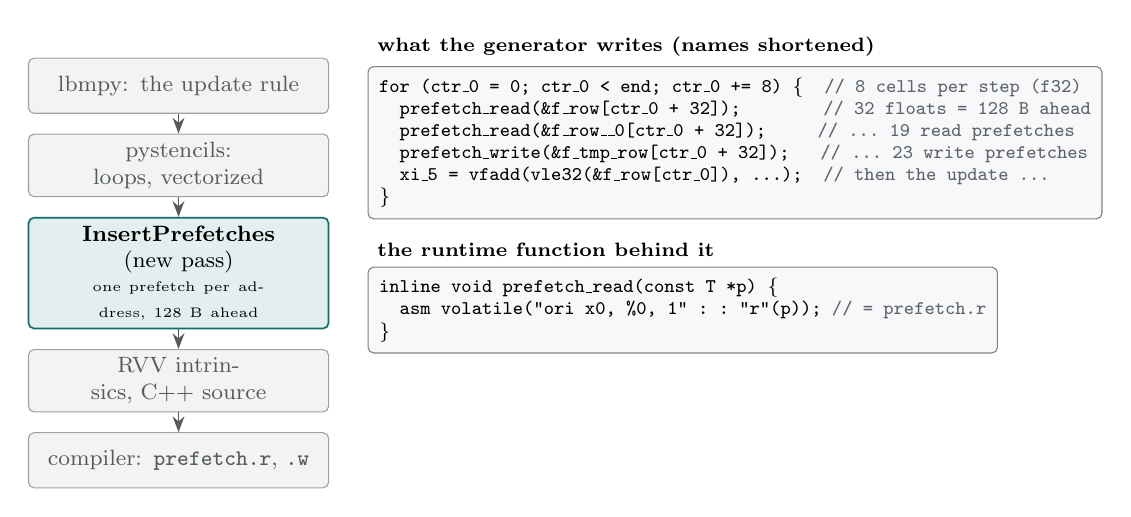
\begin{tikzpicture}
  \tikzset{st/.style={box,text width=36mm,font=\scriptsize,minimum height=5mm,inner sep=2pt}}
  \node[st,quiet] (b1) at (0,0) {lbmpy: the update rule};
  \node[st,quiet,below=2.5mm of b1] (b2) {pystencils: loops, vectorized};
  \node[st,added,below=2.5mm of b2] (b3) {\textbf{InsertPrefetches} (new pass)\\[-1pt]
    {\tiny one prefetch per address, 128 B ahead}};
  \node[st,quiet,below=2.5mm of b3] (b4) {RVV intrinsics, C++ source};
  \node[st,quiet,below=2.5mm of b4] (b5) {compiler: \code{prefetch.r}, \code{.w}};
  \foreach \a/\b in {b1/b2,b2/b3,b3/b4,b4/b5} \draw[arr] (\a) -- (\b);
  \node[codebox,anchor=north west] (gen) at (2.4,0.25) {%
for\ (ctr\_0\ =\ 0;\ ctr\_0\ <\ end;\ ctr\_0\ +=\ 8)\ \{\ \ \textcolor{psgray}{//\ 8\ cells\ per\ step\ (f32)}\\
\ \ prefetch\_read(\&f\_row[ctr\_0\ +\ 32]);\ \ \ \ \ \ \ \ \textcolor{psgray}{//\ 32\ floats\ =\ 128\ B\ ahead}\\
\ \ prefetch\_read(\&f\_row\_\_0[ctr\_0\ +\ 32]);\ \ \ \ \ \textcolor{psgray}{//\ ...\ 19\ read\ prefetches}\\
\ \ prefetch\_write(\&f\_tmp\_row[ctr\_0\ +\ 32]);\ \ \ \textcolor{psgray}{//\ ...\ 23\ write\ prefetches}\\
\ \ xi\_5\ =\ vfadd(vle32(\&f\_row[ctr\_0]),\ ...);\ \ \textcolor{psgray}{//\ then\ the\ update\ ...}\\
\}};
  \node[font=\scriptsize\bfseries,anchor=south west] at (gen.north west) {what the generator writes (names shortened)};
  \node[codebox,anchor=north west] (rt) at ([yshift=-6mm]gen.south west) {%
inline\ void\ prefetch\_read(const\ T\ *p)\ \{\\
\ \ asm\ volatile("ori\ x0,\ \%0,\ 1"\ :\ :\ "r"(p));\ \textcolor{psgray}{//\ =\ prefetch.r}\\
\}};
  \node[font=\scriptsize\bfseries,anchor=south west] at (rt.north west) {the runtime function behind it};
\end{tikzpicture}


  \vspace{2mm}
  {\scriptsize\color{psgray}Per build: \code{-{}-prefetch-distance=128} sets pystencils' option
  \code{cpu.vectorize.prefetch\_distance}. Main loop: 42 prefetches, one per stream; whole program: 103.
  Cores without the prefetch extension skip the instruction.\par}
  \takeaway{One new pass in pystencils: every vectorized loop prefetches all its streams.}
\end{frame}

% -----------------------------------------------------------------------------
%  The instruction behind prefetch_read / prefetch_write. Sources: figures/zicbop.tex (encoding checked
%  with GCC 16.2.1 + llvm-objdump on the laptop; runtime code from include/pystencils_runtime/rvv.hpp:
%  144-160); X60 ISA string without zicbop: docs/notes3/rvv-8x-speedup-progress-fable5.2.md (board facts);
%  176 -> 90 cycles per line: board-logs/board/streams-pattern.log (stream-test slide).
\begin{frame}{Software prefetch: the RISC-V instruction behind it}
  \begin{columns}[T,onlytextwidth]
    \column{0.56\textwidth}
    % Slide "Software prefetch: the RISC-V instruction behind it".
% Top: the 32-bit word of prefetch.r 0(a0) = ori x0, a0, 1 = 0x00156013. Fields (bit 31 on the left):
% imm[11:5] = offset/32 (here 0), imm[4:0] = type (0 = prefetch.i, 1 = prefetch.r, 3 = prefetch.w),
% rs1 = a0 = x10 = 01010, funct3 = 110 (ORI), rd = x0, opcode = 0010011 (OP-IMM: arithmetic with a
% constant). Checked on the laptop: riscv64-linux-gnu-g++ 16.2.1 -O3 -march=rv64gcv -c, then
% llvm-objdump -d prints "00156013  prefetch.r 0x0(a0)" for asm volatile("ori x0, %0, 1").
% Middle: the two readings of the same word. "X60 runs it": the stream test 176 -> 90 cycles per line
% with pfr=128 (board-logs/board/streams-pattern.log); notes3 progress log: the X60's ISA string lists
% zicbom and zicboz but not zicbop.
% Bottom: include/pystencils_runtime/rvv.hpp:144-151 (submodules/pystencils/src/pystencils/), shortened
% (comments added). GCC 16.2.1 with -march=rv64gcv compiles __builtin_prefetch to nothing, with
% -march=rv64gcv_zicbop to prefetch.r/prefetch.w (checked on the laptop; notes3 says the same of GCC 14).
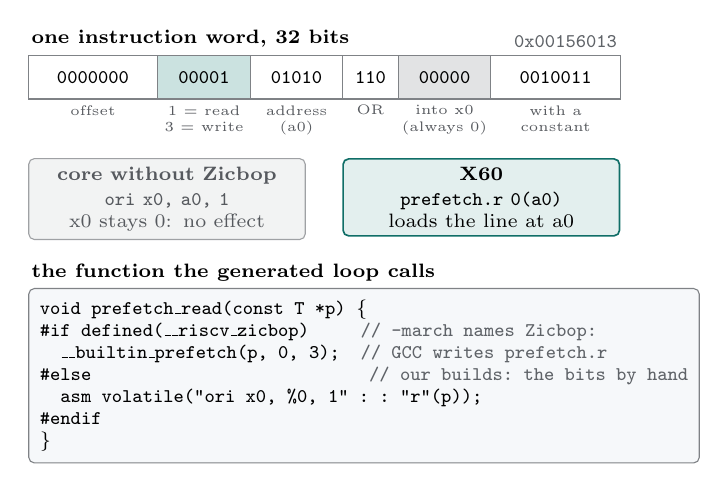
\begin{tikzpicture}
  \def\bw{2.35mm}   % width of one bit
  \def\bh{5.5mm}    % height of the word
  % field: first bit from the left (0 = bit 31) / number of bits / bits / label below / fill
  \foreach \s/\n/\bits/\lab/\fil in {
      0/7/0000000/{offset}/white,
      7/5/00001/{1 = read\\3 = write}/psteal!22,
      12/5/01010/{address\\(a0)}/white,
      17/3/110/{OR}/white,
      20/5/00000/{into x0\\(always 0)}/psgray!18,
      25/7/0010011/{with a\\constant}/white} {
    \draw[psgray!80,fill=\fil] (\s*\bw,0) rectangle ++(\n*\bw,\bh);
    \node[font=\ttfamily\scriptsize] at (\s*\bw+\n*\bw/2,\bh/2) {\bits};
    \node[lbl,anchor=north,font=\tiny,inner sep=1pt] at (\s*\bw+\n*\bw/2,-0.4mm) {\lab};
  }
  \node[font=\scriptsize\bfseries,anchor=south west,inner sep=1pt] at (0,\bh+0.6mm)
    {one instruction word, 32 bits};
  \node[font=\scriptsize,text=psgray,anchor=south east,inner sep=1pt] at (32*\bw,\bh+0.6mm)
    {\code{0x00156013}};
  % the two readings of the same bits
  \node[box,quiet,text width=33mm,font=\scriptsize,anchor=north west] (old) at (0,-7.5mm)
    {\textbf{core without Zicbop}\\[1pt]\code{ori x0, a0, 1}\\x0 stays 0: no effect};
  \node[box,added,text width=33mm,font=\scriptsize,anchor=north east] (new) at (32*\bw,-7.5mm)
    {\textbf{X60}\\[1pt]\code{prefetch.r 0(a0)}\\loads the line at a0};
  % the runtime function that the generated loop calls
  \node[codebox,anchor=north west] (rt) at (0,-24mm) {%
void\ prefetch\_read(const\ T\ *p)\ \{\\
\#if\ defined(\_\_riscv\_zicbop)\ \ \ \ \ \textcolor{psgray}{//\ -march\ names\ Zicbop:}\\
\ \ \_\_builtin\_prefetch(p,\ 0,\ 3);\ \ \textcolor{psgray}{//\ GCC\ writes\ prefetch.r}\\
\#else\ \ \ \ \ \ \ \ \ \ \ \ \ \ \ \ \ \ \ \ \ \ \ \ \ \ \ \textcolor{psgray}{//\ our\ builds:\ the\ bits\ by\ hand}\\
\ \ asm\ volatile("ori\ x0,\ \%0,\ 1"\ :\ :\ "r"(p));\\
\#endif\\
\}};
  \node[font=\scriptsize\bfseries,anchor=south west,inner sep=1pt] at ([yshift=0.4mm]rt.north west)
    {the function the generated loop calls};
\end{tikzpicture}

    \column{0.41\textwidth}
    \vspace{1mm}
    \begin{itemize}\small
      \item RVV has no prefetch instruction and no prefetch intrinsic. Prefetch comes from a small
            scalar extension, \term{Zicbop}: \code{prefetch.r} (will read), \code{prefetch.w} (will write).
      \item Its bits are a \term{hint}: they also spell an instruction without effect, so cores
            without Zicbop just skip it.
      \item The X60 runs Zicbop but does not list it, so our \code{-march} lacks it and GCC drops
            \code{\_\_builtin\_prefetch}. We write the bits by hand (\term{inline assembly}).
    \end{itemize}
  \end{columns}
  \takeaway{Prefetch is a scalar Zicbop hint, not RVV: safe on any core; on the X60, 176 to 90 cycles per line.}
\end{frame}

% -----------------------------------------------------------------------------
\begin{frame}{Update in place: the AA pattern}
  \vspace{1mm}
  {\small The name: the usual way reads array A and writes array B (AB). This way only uses A (AA).\par}
  \begin{columns}[T,onlytextwidth]
    \column{0.4\textwidth}
    {\small\bfseries AB pattern (before)\par}
    \vspace{3mm}
    \centering% The usual "AB" scheme: two arrays, A and B. Each step reads one and writes the other, then
% they swap roles. Shown next to the AA pattern (aa-pattern.tex), which uses only array A.
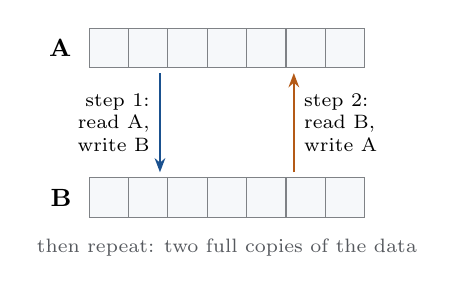
\begin{tikzpicture}[
    cell/.style={draw=psgray!80,fill=codebg,minimum width=5mm,minimum height=5mm,inner sep=0pt},
    st/.style={-{Stealth[length=1.8mm]},thick}]
  \foreach \k in {0,...,6} {
    \node[cell] at (\k*0.5+0.25,0) {};
    \node[cell] at (\k*0.5+0.25,-1.9) {};
  }
  \node[font=\small\bfseries,anchor=east] at (-0.1,0) {A};
  \node[font=\small\bfseries,anchor=east] at (-0.1,-1.9) {B};
  \draw[st,psblue!85!black] (0.9,-0.32) -- node[left,font=\scriptsize,align=right,text=black] {step 1:\\read A,\\write B} (0.9,-1.58);
  \draw[st,psorange!90!black] (2.6,-1.58) -- node[right,font=\scriptsize,align=left,text=black] {step 2:\\read B,\\write A} (2.6,-0.32);
  \node[lbl,anchor=north] at (1.75,-2.3) {then repeat: two full copies of the data};
\end{tikzpicture}


    \vspace{1mm}
    {\small\textbf{42 streams}, 260 bytes per cell\par}

    \vspace{3mm}
    {\scriptsize\color{psgray}New for AA: sweepgen kernels, their halo exchange, and wall passes for
    even and odd steps.\par}
    \column{0.56\textwidth}
    {\small\bfseries AA pattern: one array, two kinds of step\par}
    \vspace{1mm}
    \centering% Slide 12: the AA pattern for one pair of directions, east (E) and west (W), seen from cell x
% (as in lbmpy's AA accessors). Even step: read both slots of x, write each value into the
% other's slot of x. Odd step: read from the neighbours' slots, write to the neighbours' slots.
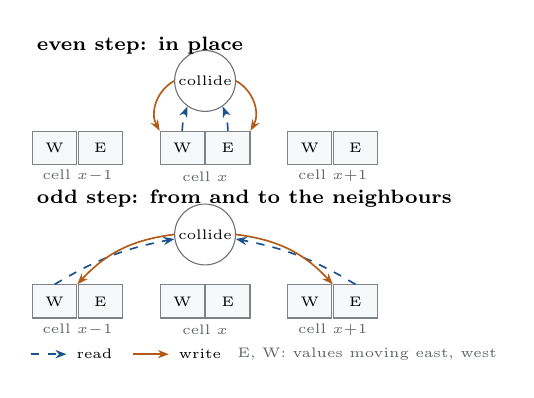
\begin{tikzpicture}[
    slot/.style={draw=psgray!80,fill=codebg,minimum width=5.6mm,minimum height=4.2mm,inner sep=0pt,font=\tiny},
    coll/.style={circle,draw=psgray!90,fill=white,inner sep=1pt,font=\tiny},
    rd/.style={-{Stealth[length=1.4mm]},semithick,draw=psblue!85!black,dashed},
    wr/.style={-{Stealth[length=1.4mm]},semithick,draw=psorange!90!black}]
  \foreach \p/\py/\ttl in {e/0/{even step: in place}, o/-1.95/{odd step: from and to the neighbours}} {
    \foreach \c/\lab in {0/$x{-}1$, 1/$x$, 2/$x{+}1$} {
      \node[slot] (\p W\c) at (\c*1.62+0.3,\py) {W};
      \node[slot] (\p E\c) at (\c*1.62+0.88,\py) {E};
      \node[font=\tiny,text=psgray] at (\c*1.62+0.59,\py-0.36) {cell \lab};
    }
    \node[coll] (\p col) at (2.21,\py+0.85) {collide};
    \node[font=\scriptsize\bfseries,anchor=west] at (-0.05,\py+1.3) {\ttl};
  }
  \draw[rd] (eE1.north) to[bend right=10] (ecol);
  \draw[rd] (eW1.north) to[bend left=10] (ecol);
  \draw[wr] (ecol.west) to[bend right=45] (eW1.north west);
  \draw[wr] (ecol.east) to[bend left=45] (eE1.north east);
  \draw[rd] (oW0.north) to[bend left=10] (ocol);
  \draw[rd] (oE2.north) to[bend right=10] (ocol);
  \draw[wr] (ocol.east) to[bend left=20] (oE2.north west);
  \draw[wr] (ocol.west) to[bend right=20] (oW0.north east);
  \draw[rd] (0,-2.62) -- ++(0.45,0) node[right,font=\tiny,text=black] {read};
  \draw[wr] (1.3,-2.62) -- ++(0.45,0) node[right,font=\tiny,text=black] {write};
  \node[font=\tiny,text=psgray,anchor=west] at (2.5,-2.62) {E, W: values moving east, west};
\end{tikzpicture}


    \vspace{1mm}
    {\small\textbf{23 streams}, 184 bytes per cell\par}
  \end{columns}
  \takeaway{Whole program, with prefetch, f32 / f64: GCC \sx{1.43} / \sx{1.60}, Clang \sx{1.47} / \sx{1.68}.}
\end{frame}

% -----------------------------------------------------------------------------
%  The split loop (build explicit_cse_aa_split). Sources: figures/split-loop.tex (lbm_split.py, the
%  generated driver, block and scratch sizes). The split loop is always in place (AA): --split needs
%  --streaming-pattern=aa (SweepgenLdcCPU.py:100-102).
\begin{frame}{The split loop: the same update in eight short passes}
  \vspace{5mm}
  \centering% Slide "The split loop: the same update in eight short passes".
% Source: submodules/walberla/apps/benchmarks/SweepgenLbmCPU/lbm_split.py (class SplitAA), used by
% SweepgenLdcCPU (--split=BY,GM,GP; CMakeLists.txt:63-70: f32 2,5,3, f64 1,5,3). For each block of BY
% rows of one z-plane the generated driver LBM_SPLIT::streamCollide calls 8 passes (generated
% SweepgenLdcCPU.cpp of explicit_cse_aa_split, e.g. build/presentation4-x86/gcc-f32/.../gen/
% SweepgenLdcCPU.cpp:6933-6997): m0..m3 add up mass and momentum of 5, 5, 5, 4 values into the scratch
% acc; macro computes rho, u (into the scratch scr, and into the outputs); c0..c2 reload 7, 6, 6
% values (the rest value and 3 opposite pairs, then 3 pairs, 3 pairs), collide (relax) them and store them in
% place. Arrays per pass: 5 / 4 outputs / 7 or 6 (plus the scratch, which stays in L1).
% Block size, 64^3 block: f32 19 x 2 rows x 64 cells x 4 B = 9728 B; f64 19 x 1 x 64 x 8 B = 9728 B.
% Scratch (driver): 9 x sc values, sc = 128 (f32) / 64 (f64): 4608 B. L1 data cache 32 KB.
% The one-loop row: the in-place (AA) StreamCollide kernel: 19 + 4 = 23 arrays (see stream-def).
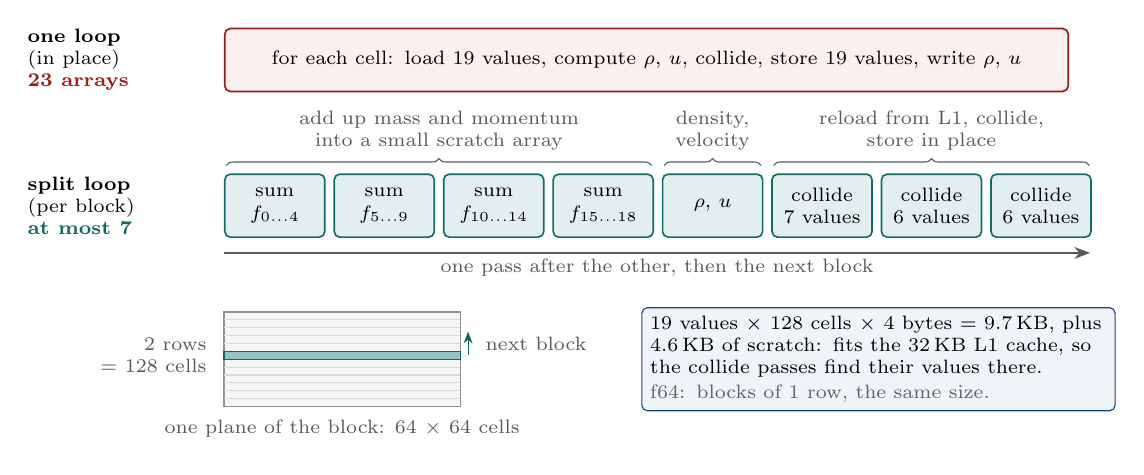
\begin{tikzpicture}[x=1mm,y=1mm]
  \tikzset{pass/.style={added,minimum height=8mm,text width=12mm,inner sep=1pt,font=\scriptsize},
           rowlbl/.style={font=\scriptsize,align=left,anchor=west,inner sep=0pt},
           tag/.style={font=\scriptsize,align=center,anchor=west,inner sep=1pt}}
  % ---- before: one loop over all cells, all 19 values at once
  %   row labels: what, and how many arrays it walks through at once
  \node[rowlbl] at (0,0) {\textbf{one loop}\\(in place)\\\textcolor{psred!85!black}{\textbf{23 arrays}}};
  \node[wrong,anchor=west,minimum height=8mm,text width=105mm,font=\scriptsize] (one) at (25,0)
    {for each cell: load 19 values, compute $\rho$, $u$, collide, store 19 values, write $\rho$, $u$};
  % ---- split loop: 8 passes over one block
  \node[rowlbl] at (0,-18.5) {\textbf{split loop}\\(per block)\\\textcolor{psteal!85!black}{\textbf{at most 7}}};
  \foreach \k/\t in {0/{sum\\$f_{0\ldots4}$},1/{sum\\$f_{5\ldots9}$},2/{sum\\$f_{10\ldots14}$},
                     3/{sum\\$f_{15\ldots18}$},4/{$\rho$, $u$},5/{collide\\7 values},
                     6/{collide\\6 values},7/{collide\\6 values}}
    \node[pass,anchor=west] (p\k) at (25+\k*13.9,-18.5) {\t};
  \draw[arr] (25,-24.5) -- (135,-24.5) node[pos=0.5,below=-0.5mm,lbl] {one pass after the other, then the next block};
  % ---- what the groups of passes do
  \foreach \a/\b/\t in {p0/p3/{add up mass and momentum\\into a small scratch array},
                        p4/p4/{density,\\velocity},
                        p5/p7/{reload from L1, collide,\\store in place}}
    \draw[decorate,decoration={brace,amplitude=2.5pt},psgray!90!black]
      ([xshift=0.3mm,yshift=1mm]\a.north west) -- ([xshift=-0.3mm,yshift=1mm]\b.north east)
      node[midway,above=2pt,lbl] {\t};
  % ---- the block: 2 rows of one plane
  \begin{scope}[shift={(25,-44)}]
    \draw[psgray!70,fill=psgray!6] (0,0) rectangle (30,12);
    \foreach \r in {1,...,11} \draw[psgray!25] (0,\r) -- (30,\r);
    \draw[psteal!85!black,fill=psteal!45] (0,6) rectangle (30,7);
    \draw[-{Stealth[length=1.5mm]},psteal!85!black] (31,6.5) -- (31,9.5);
    \node[lbl,anchor=west,align=left] at (32,8) {next block};
    \node[lbl,anchor=north] at (15,-0.5) {one plane of the block: 64 $\times$ 64 cells};
    \node[lbl,anchor=east,align=right] at (-1,6.5) {2 rows\\= 128 cells};
  \end{scope}
  \node[info,anchor=west,text width=58mm,font=\scriptsize,align=left] at (78,-38)
    {19 values $\times$ 128 cells $\times$ 4 bytes = 9.7\,KB, plus 4.6\,KB of scratch: fits the
     32\,KB L1 cache, so the collide passes find their values there.\\[1pt]
     {\color{psgray}f64: blocks of 1 row, the same size.}};
\end{tikzpicture}

  \takeaway{Each pass walks through at most 7 arrays, and the collide passes find their values in the L1
    cache.}
\end{frame}

% -----------------------------------------------------------------------------
%  Why the split build has no software prefetch. Late lines (l2_miss per cell update, GCC f32, 64^3,
%  streams-ldc.log via scripts/presentation4/streams_table.py): explicit_cse_aa 1.762, explicit_cse_aa_split
%  0.341, neither with software prefetch (0 hint instructions). Prefetch added to the split loop: kernel
%  lab, periodic box 64^3, GCC, the generated split passes with cpu.vectorize.prefetch_distance=128
%  (docs/notes3/board-logs/lab7.log, best of 3 rounds): f32 BY=2 GM=5 GP=3 9.967 -> 9.255 MLUP/s (-7.1 %),
%  instructions per cell 66.4 -> 88.0 (+33 %); f64 BY=1 5.528 -> 4.802 (-13.1 %), 114.5 -> 159.8 (+40 %).
%  Report 3 (r03, section "Fewer streams") says the same of the hand-written split kernel. Gains in the
%  takeaway: slide_numbers.py, "split loop (instead of prefetch)": 1.171 / 1.211 / 1.219 / 1.221.
\begin{frame}{The split loop in code, and why it needs no prefetch}
  \begin{columns}[T,onlytextwidth]
    \column{0.57\textwidth}
    \vspace{0.5mm}
    % Slide "The split loop in code, and why it needs no prefetch".
% Top: the generated driver LBM_SPLIT::streamCollide (lbm_split.py driver_code; generated
% SweepgenLdcCPU.cpp of explicit_cse_aa_split, e.g. build/presentation4-x86/gcc-f32/apps/benchmarks/
% SweepgenLdcCPU/_gen/SweepgenLdcCPU_explicit_cse_aa_split/gen/SweepgenLdcCPU.cpp:6933-6997), f32 (2 rows
% per block), even step with output, shortened: argument lists cut to the arrays, the odd step and the
% no-output flavour dropped. Bottom: pass m1_0 of the same file (lines 4443-4540), shortened: the y
% and z momentum and the remainder loop left out, indexing written as f5[y][x]. That file is the x86
% build (AVX loads); the board's RVV build has the same passes with RVV loads (vle32 = __riscv_vle32_v_f32m1).
% D3Q19 in lbmpy's order: c_x of values 7, 8, 9 is -1, +1, -1, so x-momentum gets v8 - v7 - v9.
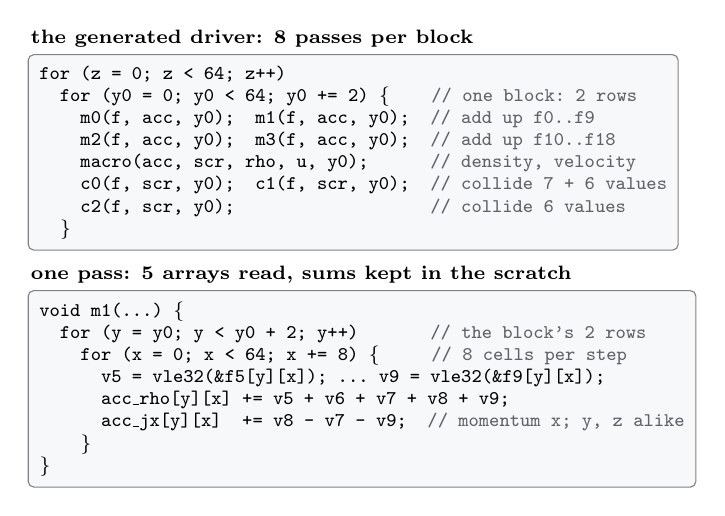
\begin{tikzpicture}
  \node[codebox,anchor=north west] (drv) at (0,0) {%
for\ (z\ =\ 0;\ z\ <\ 64;\ z++)\\
\ \ for\ (y0\ =\ 0;\ y0\ <\ 64;\ y0\ +=\ 2)\ \{\ \ \ \ \textcolor{psgray}{//\ one\ block:\ 2\ rows}\\
\ \ \ \ m0(f,\ acc,\ y0);\ \ m1(f,\ acc,\ y0);\ \ \textcolor{psgray}{//\ add\ up\ f0..f9}\\
\ \ \ \ m2(f,\ acc,\ y0);\ \ m3(f,\ acc,\ y0);\ \ \textcolor{psgray}{//\ add\ up\ f10..f18}\\
\ \ \ \ macro(acc,\ scr,\ rho,\ u,\ y0);\ \ \ \ \ \ \textcolor{psgray}{//\ density,\ velocity}\\
\ \ \ \ c0(f,\ scr,\ y0);\ \ c1(f,\ scr,\ y0);\ \ \textcolor{psgray}{//\ collide\ 7\ +\ 6\ values}\\
\ \ \ \ c2(f,\ scr,\ y0);\ \ \ \ \ \ \ \ \ \ \ \ \ \ \ \ \ \ \ \textcolor{psgray}{//\ collide\ 6\ values}\\
\ \ \}};
  \node[font=\scriptsize\bfseries,anchor=south west,inner sep=1pt] at ([yshift=0.4mm]drv.north west)
    {the generated driver: 8 passes per block};
  \node[codebox,anchor=north west] (pass) at ([yshift=-5mm]drv.south west) {%
void\ m1(...)\ \{\\
\ \ for\ (y\ =\ y0;\ y\ <\ y0\ +\ 2;\ y++)\ \ \ \ \ \ \ \textcolor{psgray}{//\ the\ block's\ 2\ rows}\\
\ \ \ \ for\ (x\ =\ 0;\ x\ <\ 64;\ x\ +=\ 8)\ \{\ \ \ \ \ \textcolor{psgray}{//\ 8\ cells\ per\ step}\\
\ \ \ \ \ \ v5\ =\ vle32(\&f5[y][x]);\ ...\ v9\ =\ vle32(\&f9[y][x]);\\
\ \ \ \ \ \ acc\_rho[y][x]\ +=\ v5\ +\ v6\ +\ v7\ +\ v8\ +\ v9;\\
\ \ \ \ \ \ acc\_jx[y][x]\ \ +=\ v8\ -\ v7\ -\ v9;\ \ \textcolor{psgray}{//\ momentum\ x;\ y,\ z\ alike}\\
\ \ \ \ \}\\
\}};
  \node[font=\scriptsize\bfseries,anchor=south west,inner sep=1pt] at ([yshift=0.4mm]pass.north west)
    {one pass: 5 arrays read, sums kept in the scratch};
\end{tikzpicture}

    \column{0.41\textwidth}
    \vspace{1mm}
    {\small\bfseries Why no software prefetch\par}
    \vspace{1mm}
    \begin{itemize}\small
      \item At most 7 arrays per pass: the \term{hardware prefetcher} keeps up. Late lines per cell:
            1.8 in place, 0.34 split (no prefetch in either).
      \item The collide passes reload lines that are still in L1.
      \item Tried: with prefetch the split loop is 7\,\% (f32) and 13\,\% (f64) slower, from 33\,\% and
            40\,\% more instructions.
    \end{itemize}
    \vspace{1mm}
    {\scriptsize\color{psgray}Last point: kernel lab, periodic box, GCC.\par}
  \end{columns}
  \takeaway{Split loop against in place + prefetch, one core, f32 / f64: GCC \sx{1.17} / \sx{1.21}, Clang \sx{1.22} / \sx{1.22}.}
\end{frame}

% =============================================================================
\section{Results and limits}

%  The result figures: speedup (one plot per precision) and MLUP/s are separate figures, one core
%  first, then several cores. All numbers: scripts/presentation4/slide_numbers.py --tex (see the figures).
%  Second session: scripts/presentation4/speedup_check.sh (board 19:11-19:28, 3 interleaved rounds; logs
%  board-logs/board/speedup-*.log). Today / all.sh, best of 3: scalar GCC f32 0.901, Clang f32 0.919, GCC f64
%  0.989, Clang f64 1.042; aa_pf 0.999 to 1.013; split 0.965 to 1.001. Speedups today (all.sh): GCC f32 aa_pf
%  5.274 (4.738), split 6.119 (5.548); Clang f32 4.947 (4.551), 6.045 (5.550); GCC f64 4.315 (4.230), 5.000
%  (5.123); Clang f64 3.944 (4.061), 4.698 (4.959).
\begin{frame}{Results: the whole program on one core, f32}
  \vspace{1mm}
  \centering% Slide "Results: one core, f32": whole-program speedup over the plain scalar build of the same
% compiler, lid-driven cavity (SweepgenLdcCPU), f32, 64^3 cells, one core, best of 3 runs of 200 steps.
% One session (board, scripts/presentation4/all.sh, logs docs/presentation4/board-logs/board/
% ldc-{gcc,clang}-{scalar,autovec,rvv}-f32-1core.log), printed by
%   python3 scripts/presentation4/slide_numbers.py --tex docs/presentation4/board-logs/board
% Bars and numbers: GCC 14.2. Diamonds, right of each bar: Clang 18.1 against its own plain scalar.
% Groups (style onecore, preamble of slides.tex): plain = scalar, plainav = autovec,
% best = scalar_cse_aa, bestav = autovec_cse_aa (auto-vectorized: hatched), rvv = explicit_cse,
% pf = explicit_cse_pf, aa = explicit_cse_aa_pf, split = explicit_cse_aa_split (no software prefetch: 0 hints).
% The MLUP/s of the same runs: figures/mlups-1core.tex. Same y scale as speedup-1core-f64.tex.
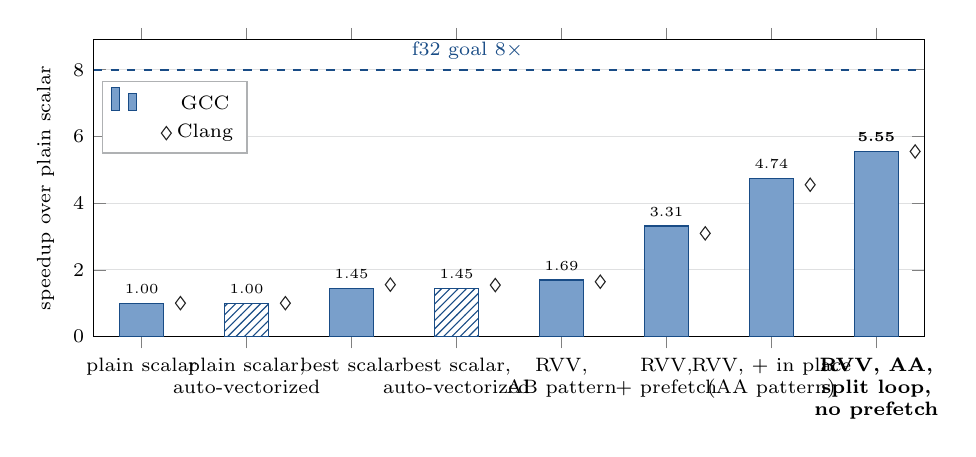
\begin{tikzpicture}
  \begin{axis}[onecore, ybar, bar width=16pt, height=5.35cm, ymax=8.9,
      ylabel={speedup over plain scalar},
      nodes near coords style={font=\tiny,anchor=south},
      legend style={at={(0.01,0.86)},anchor=north west}]
    \addplot[fill=psblue!60,draw=psblue!80!black,bar shift=0pt] coordinates {
      (plain,1.000)[1.00] (best,1.447)[1.45] (rvv,1.693)[1.69] (pf,3.313)[3.31] (aa,4.738)[4.74]
      (split,5.548)[\textbf{5.55}]};
    \addplot[clang1,clang1legend,xshift=14pt] coordinates {
      (plain,1.000) (plainav,0.999) (best,1.554) (bestav,1.542) (rvv,1.642) (pf,3.093) (aa,4.551)
      (split,5.550)};
    \addplot[pattern=north east lines,pattern color=psblue!80!black,draw=psblue!80!black,
      bar shift=0pt,forget plot] coordinates {(plainav,0.997)[1.00] (bestav,1.449)[1.45]};
    \legend{GCC, Clang}
    \draw[psblue!80!black,dashed,thick] (axis description cs:0,8/8.9) -- (axis description cs:1,8/8.9)
      node[pos=0.45,above,font=\scriptsize] {f32 goal \sx{8}};
  \end{axis}
\end{tikzpicture}


  \vspace{0.5mm}
  {\scriptsize\color{psgray}Bars and numbers: GCC; diamonds: Clang. Each compiler against its own plain
  scalar build. Hatched: auto-vectorized. $64^3$ cells, best of 3 runs of 200 steps. A second session,
  interleaved runs: RVV builds within 1\,\%, plain scalar 8 to 10\,\% slower, so f32 speedups 9 to 11\,\% higher.\par}
  \takeaway{f32 reaches \sx{5.55} of the possible \sx{8} with both compilers. Auto-vectorization gives
    nothing.}
\end{frame}

% -----------------------------------------------------------------------------
\begin{frame}{Results: the whole program on one core, f64}
  \vspace{1mm}
  \centering% Slide "Results: one core, f64": whole-program speedup over the plain scalar build of the same
% compiler, lid-driven cavity (SweepgenLdcCPU), f64, 64^3 cells, one core, best of 3 runs of 200 steps.
% One session (board, scripts/presentation4/all.sh, logs docs/presentation4/board-logs/board/
% ldc-{gcc,clang}-{scalar,autovec,rvv}-f64-1core.log), printed by
%   python3 scripts/presentation4/slide_numbers.py --tex docs/presentation4/board-logs/board
% Bars and numbers: GCC 14.2. Diamonds, right of each bar: Clang 18.1 against its own plain scalar.
% Groups (style onecore, preamble of slides.tex): plain = scalar, plainav = autovec,
% best = scalar_cse_aa, bestav = autovec_cse_aa (auto-vectorized: hatched), rvv = explicit_cse,
% pf = explicit_cse_pf, aa = explicit_cse_aa_pf, split = explicit_cse_aa_split (no software prefetch: 0 hints).
% The MLUP/s of the same runs: figures/mlups-1core.tex. Same y scale as speedup-1core-f32.tex.
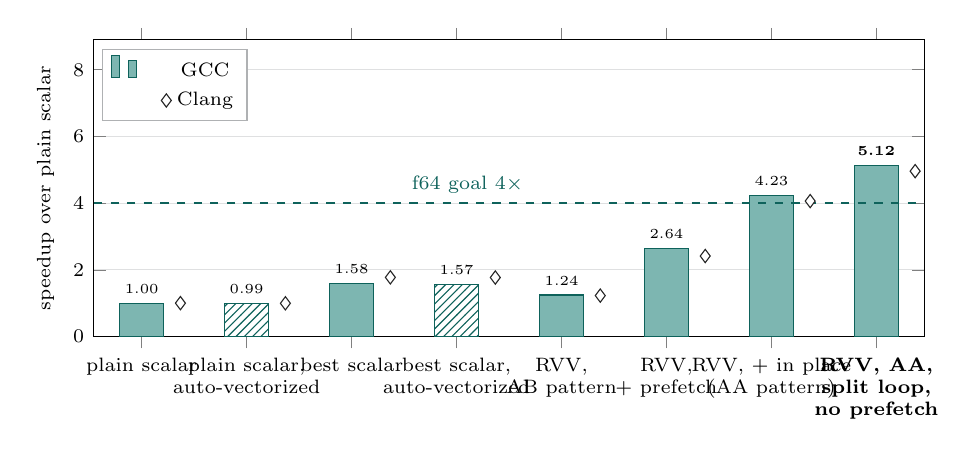
\begin{tikzpicture}
  \begin{axis}[onecore, ybar, bar width=16pt, height=5.35cm, ymax=8.9,
      ylabel={speedup over plain scalar},
      nodes near coords style={font=\tiny,anchor=south},
      legend style={at={(0.01,0.97)},anchor=north west}]
    \addplot[fill=psteal!55,draw=psteal!80!black,bar shift=0pt] coordinates {
      (plain,1.000)[1.00] (best,1.585)[1.58] (rvv,1.243)[1.24] (pf,2.637)[2.64] (aa,4.230)[4.23]
      (split,5.123)[\textbf{5.12}]};
    \addplot[clang1,clang1legend,xshift=14pt] coordinates {
      (plain,1.000) (plainav,0.995) (best,1.773) (bestav,1.768) (rvv,1.226) (pf,2.413) (aa,4.061)
      (split,4.959)};
    \addplot[pattern=north east lines,pattern color=psteal!80!black,draw=psteal!80!black,
      bar shift=0pt,forget plot] coordinates {(plainav,0.987)[0.99] (bestav,1.566)[1.57]};
    \legend{GCC, Clang}
    \draw[psteal!80!black,dashed,thick] (axis description cs:0,4/8.9) -- (axis description cs:1,4/8.9)
      node[pos=0.45,above,font=\scriptsize] {f64 goal \sx{4}};
  \end{axis}
\end{tikzpicture}


  \vspace{0.5mm}
  {\scriptsize\color{psgray}Bars and numbers: GCC; diamonds: Clang. Each compiler against its own plain
  scalar build. Hatched: auto-vectorized. $64^3$ cells, best of 3 runs of 200 steps. A second session,
  interleaved runs: f64 speedups 5\,\% lower to 2\,\% higher; split loop \sx{5.00} (GCC), \sx{4.70} (Clang).\par}
  \takeaway{f64 passes its \sx{4} goal with both compilers: \sx{5.12} with GCC, \sx{4.96} with Clang
    (split loop).}
\end{frame}

% -----------------------------------------------------------------------------
\begin{frame}{One core: the measured speed}
  \vspace{1mm}
  \centering% Slide "One core: MLUP/s": million cell updates per second of the whole program, lid-driven cavity
% (SweepgenLdcCPU), 64^3 cells, one core, best of 3 runs of 200 steps. One session (board,
% scripts/presentation4/all.sh, logs docs/presentation4/board-logs/board/
% ldc-{gcc,clang}-{scalar,autovec,rvv}-{f32,f64}-1core.log), printed by
%   python3 scripts/presentation4/slide_numbers.py --tex docs/presentation4/board-logs/board
% Bars and numbers: GCC 14.2, f32 (blue) and f64 (teal). Diamonds: Clang 18.1, on the outer side of
% the bar of the same precision (f32 left, f64 right).
% Groups (style onecore, preamble of slides.tex): plain = scalar, plainav = autovec,
% best = scalar_cse_aa, bestav = autovec_cse_aa (auto-vectorized: hatched), rvv = explicit_cse,
% pf = explicit_cse_pf, aa = explicit_cse_aa_pf, split = explicit_cse_aa_split (no software prefetch: 0 hints).
% The speedups of the same runs: figures/speedup-1core-{f32,f64}.tex.
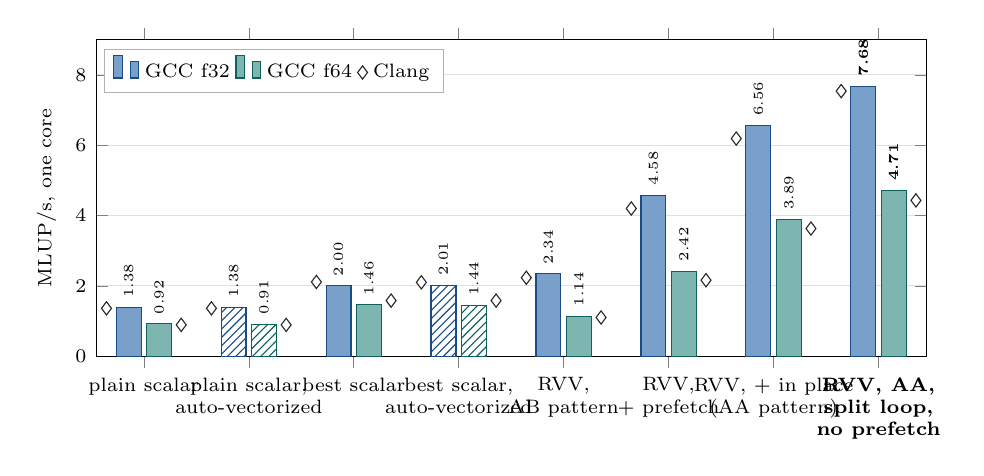
\begin{tikzpicture}
  \begin{axis}[onecore, ybar, bar width=9pt, height=5.6cm, ymax=9,
      ylabel={MLUP/s, one core},
      nodes near coords style={font=\tiny,rotate=90,anchor=west},
      legend style={at={(0.01,0.97)},anchor=north west}, legend columns=3]
    \addplot[fill=psblue!60,draw=psblue!80!black,bar shift=-5.5pt] coordinates {
      (plain,1.38)[1.38] (best,2.00)[2.00] (rvv,2.34)[2.34] (pf,4.58)[4.58] (aa,6.56)[6.56]
      (split,7.68)[\textbf{7.68}]};
    \addplot[fill=psteal!55,draw=psteal!80!black,bar shift=5.5pt] coordinates {
      (plain,0.92)[0.92] (best,1.46)[1.46] (rvv,1.14)[1.14] (pf,2.42)[2.42] (aa,3.89)[3.89]
      (split,4.71)[\textbf{4.71}]};
    \addplot[clang1,clang1legend,xshift=-13.5pt] coordinates {
      (plain,1.36) (plainav,1.36) (best,2.11) (bestav,2.10) (rvv,2.23) (pf,4.20) (aa,6.19) (split,7.54)};
    \addplot[clang1,xshift=13.5pt,forget plot] coordinates {
      (plain,0.89) (plainav,0.89) (best,1.58) (bestav,1.58) (rvv,1.10) (pf,2.16) (aa,3.63) (split,4.43)};
    \addplot[pattern=north east lines,pattern color=psblue!80!black,draw=psblue!80!black,
      bar shift=-5.5pt,forget plot] coordinates {(plainav,1.38)[1.38] (bestav,2.01)[2.01]};
    \addplot[pattern=north east lines,pattern color=psteal!80!black,draw=psteal!80!black,
      bar shift=5.5pt,forget plot] coordinates {(plainav,0.91)[0.91] (bestav,1.44)[1.44]};
    \legend{GCC f32, GCC f64, Clang}
  \end{axis}
\end{tikzpicture}


  \vspace{0.5mm}
  {\scriptsize\color{psgray}MLUP/s: million cell updates per second. Bars and numbers: GCC; diamonds:
  Clang, next to the bar of the same precision. Hatched: auto-vectorized. $64^3$ cells, best of 3 runs
  of 200 steps.\par}
  \takeaway{Fastest build (split loop), f32 / f64: GCC 7.68 / 4.71, Clang 7.54 / 4.43 MLUP/s.}
\end{frame}

% -----------------------------------------------------------------------------
\begin{frame}{Several cores: speedup over plain scalar}
  \vspace{1mm}
  \centering% Slide "Several cores: speedup over plain scalar", left panel: f32. Speedup over the plain scalar
% build of the same compiler at the same core count, lid-driven cavity (SweepgenLdcCPU), one 64^3
% block per MPI process, best of 3 runs of 200 steps. One session (board, scripts/presentation4/all.sh,
% logs docs/presentation4/board-logs/board/ldc-{gcc,clang}-{scalar,autovec,rvv}-f32-{1,4,8}core.log),
% printed by
%   python3 scripts/presentation4/slide_numbers.py --tex docs/presentation4/board-logs/board
% Bars and numbers: GCC 14.2. Diamonds: Clang 18.1, against its own plain scalar (plain scalar = 1
% for both compilers, so no diamond there). Series as figures/mlups-multicore.tex: plain scalar =
% scalar, best scalar = scalar_cse_aa, auto-vec. in place = autovec_cse_aa (hatched),
% RVV in place + prefetch = explicit_cse_aa_pf, RVV split loop = explicit_cse_aa_split (in place,
% no software prefetch: 0 hints).
% Styles mc, pl, bs, av, rv, sp, cl: preamble of slides.tex. Same ymax as speedup-multicore-f64.tex.
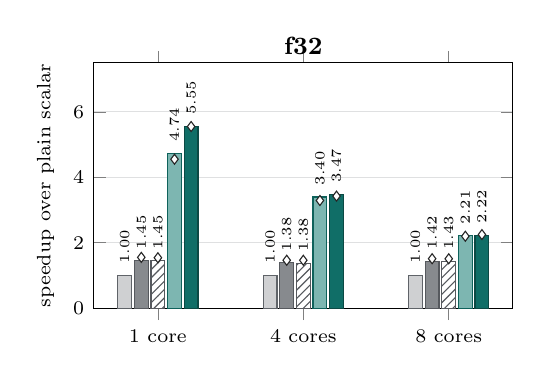
\begin{tikzpicture}
  \begin{axis}[mc, ymax=7.5, title={f32}, ylabel={speedup over plain scalar}]
    \addplot[pl] coordinates {(1,1)[1.00] (4,1)[1.00] (8,1)[1.00]};
    \addplot[bs] coordinates {(1,1.447)[1.45] (4,1.384)[1.38] (8,1.425)[1.42]};
    \addplot[av] coordinates {(1,1.449)[1.45] (4,1.379)[1.38] (8,1.427)[1.43]};
    \addplot[rv] coordinates {(1,4.738)[4.74] (4,3.397)[3.40] (8,2.211)[2.21]};
    \addplot[sp] coordinates {(1,5.548)[5.55] (4,3.472)[3.47] (8,2.222)[2.22]};
    \addplot[cl,xshift=-6pt] coordinates {(1,1.554) (4,1.466) (8,1.513)};
    \addplot[cl,xshift=0pt] coordinates {(1,1.542) (4,1.466) (8,1.511)};
    \addplot[cl,xshift=6pt] coordinates {(1,4.551) (4,3.290) (8,2.200)};
    \addplot[cl,xshift=12pt] coordinates {(1,5.550) (4,3.425) (8,2.250)};
  \end{axis}
\end{tikzpicture}
\hspace{0.6cm}% Slide "Several cores: speedup over plain scalar", right panel: f64. Speedup over the plain scalar
% build of the same compiler at the same core count, lid-driven cavity (SweepgenLdcCPU), one 64^3
% block per MPI process, best of 3 runs of 200 steps. One session (board, scripts/presentation4/all.sh,
% logs docs/presentation4/board-logs/board/ldc-{gcc,clang}-{scalar,autovec,rvv}-f64-{1,4,8}core.log),
% printed by
%   python3 scripts/presentation4/slide_numbers.py --tex docs/presentation4/board-logs/board
% Bars and numbers: GCC 14.2. Diamonds: Clang 18.1, against its own plain scalar (plain scalar = 1
% for both compilers, so no diamond there). Series as figures/mlups-multicore.tex.
% Styles mc, pl, bs, av, rv, sp, cl, cllegend: preamble of slides.tex. Same ymax as the f32 panel.
% The legend is stored as mcspeeduplegend and placed under both panels by \ref in slides.tex.
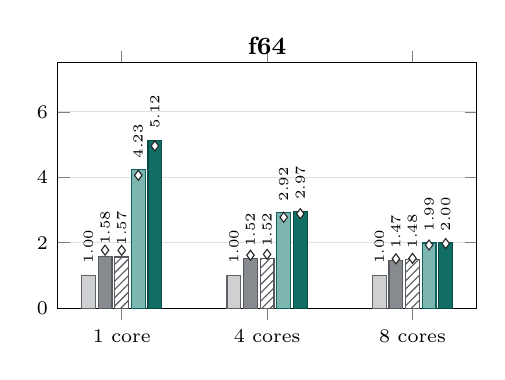
\begin{tikzpicture}
  \begin{axis}[mc, ymax=7.5, title={f64},
      legend to name=mcspeeduplegend, legend columns=-1,
      legend style={font=\tiny,draw=psgray!50,/tikz/every even column/.append style={column sep=5pt}}]
    \addplot[pl] coordinates {(1,1)[1.00] (4,1)[1.00] (8,1)[1.00]};
    \addplot[bs] coordinates {(1,1.585)[1.58] (4,1.522)[1.52] (8,1.469)[1.47]};
    \addplot[av] coordinates {(1,1.566)[1.57] (4,1.524)[1.52] (8,1.476)[1.48]};
    \addplot[rv] coordinates {(1,4.230)[4.23] (4,2.917)[2.92] (8,1.993)[1.99]};
    \addplot[sp] coordinates {(1,5.123)[5.12] (4,2.968)[2.97] (8,2.004)[2.00]};
    \addplot[cl,xshift=-6pt] coordinates {(1,1.773) (4,1.619) (8,1.510)};
    \addplot[cl,xshift=0pt] coordinates {(1,1.768) (4,1.648) (8,1.524)};
    \addplot[cl,xshift=6pt] coordinates {(1,4.061) (4,2.779) (8,1.931)};
    \addplot[cl,xshift=12pt,forget plot=false,cllegend] coordinates {(1,4.959) (4,2.887) (8,1.976)};
    \legend{plain scalar, best scalar, auto-vec.\ in place, RVV in place + prefetch, RVV split loop,
      Clang}
  \end{axis}
\end{tikzpicture}


  \vspace{0.5mm}
  \ref{mcspeeduplegend}

  \vspace{1mm}
  {\scriptsize\color{psgray}Each build against the plain scalar build of the same compiler and core
  count. Bars and numbers: GCC; diamonds: Clang. Each core runs one process with its own $64^3$ block.
  One session, best of 3 runs of 200 steps.\par}
  \takeaway{The gain shrinks with more cores. 8 cores, GCC: RVV is \sx{2.22} (f32) and \sx{2.00}
    (f64) the plain scalar build, \sx{1.56} and \sx{1.36} the best scalar build.}
\end{frame}

% -----------------------------------------------------------------------------
\begin{frame}{Several cores: the shared memory becomes the limit}
  \vspace{1mm}
  \centering% Slide "Several cores: the shared memory becomes the limit": MLUP/s of all cores together, lid-driven cavity (SweepgenLdcCPU), one 64^3 block
% per MPI process, best of 3 runs of 200 steps. 1, 4 and 8 cores from one session (board,
% scripts/presentation4/all.sh, logs docs/presentation4/board-logs/board/
% ldc-{gcc,clang}-{scalar,autovec,rvv}-{f32,f64}-{1,4,8}core.log), printed by
% python3 scripts/presentation4/slide_numbers.py --tex docs/presentation4/board-logs/board
% Bars and labels: GCC 14.2. Diamonds: Clang 18.1.
% plain scalar = scalar, best scalar = scalar_cse_aa, auto-vec. in place = autovec_cse_aa
% (hatched), RVV in place + prefetch = explicit_cse_aa_pf, RVV split loop = explicit_cse_aa_split (in place,
% no software prefetch: 0 hints).
% Memory traffic of RVV in place + prefetch (184 bytes per cell in f32, 368 in f64, the AA slide's
% numbers; walls not counted), GCC: 4 cores 17.91*184 = 3.3 / 9.89*368 = 3.6 GB/s, 8 cores
% 19.40*184 = 3.6 / 10.29*368 = 3.8 GB/s. (The split loop passes over the PDFs more than once:
% its traffic per cell is not 184 bytes, so no GB/s is given for it.)
% Both panels share ymax=27 so f32 and f64 bars compare by height. The speedups of the same runs:
% figures/speedup-multicore-{f32,f64}.tex.
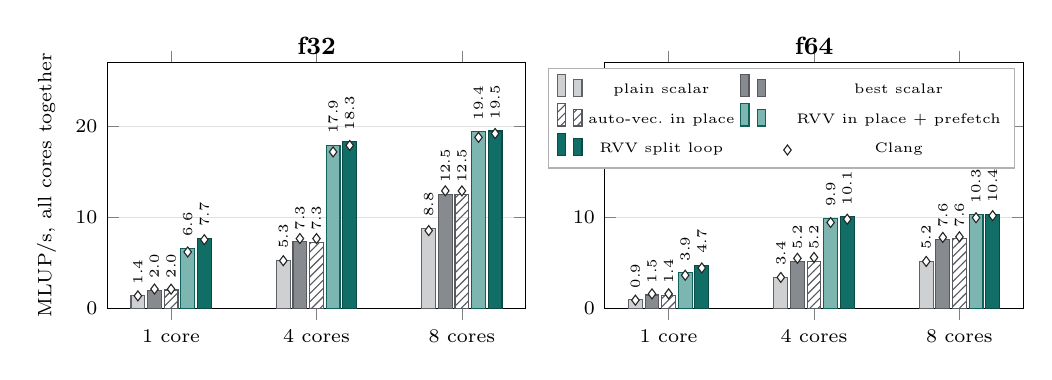
\begin{tikzpicture}
  %   Styles mc, pl, bs, av, rv, sp, cl, cllegend: preamble of slides.tex
  \begin{axis}[mc, ymax=27, name=a32, title={f32}, ylabel={MLUP/s, all cores together}]
    \addplot[pl] coordinates {(1,1.38)[1.4] (4,5.27)[5.3] (8,8.77)[8.8]};
    \addplot[bs] coordinates {(1,2.00)[2.0] (4,7.30)[7.3] (8,12.50)[12.5]};
    \addplot[av] coordinates {(1,2.01)[2.0] (4,7.27)[7.3] (8,12.52)[12.5]};
    \addplot[rv] coordinates {(1,6.56)[6.6] (4,17.91)[17.9] (8,19.40)[19.4]};
    \addplot[sp] coordinates {(1,7.68)[7.7] (4,18.31)[18.3] (8,19.49)[19.5]};
    \addplot[cl,xshift=-12pt] coordinates {(1,1.36) (4,5.23) (8,8.54)};
    \addplot[cl,xshift=-6pt] coordinates {(1,2.11) (4,7.66) (8,12.91)};
    \addplot[cl,xshift=0pt] coordinates {(1,2.10) (4,7.66) (8,12.90)};
    \addplot[cl,xshift=6pt] coordinates {(1,6.19) (4,17.19) (8,18.79)};
    \addplot[cl,xshift=12pt] coordinates {(1,7.54) (4,17.90) (8,19.21)};
  \end{axis}
  %   The legend sits in the f64 panel: its bars leave the top half free
  \begin{axis}[mc, ymax=27, at={(a32.east)}, anchor=west, xshift=1.0cm, title={f64},
      legend style={font=\tiny,at={(0.98,0.98)},anchor=north east,draw=psgray!50},
      legend columns=2]
    \addplot[pl] coordinates {(1,0.92)[0.9] (4,3.39)[3.4] (8,5.17)[5.2]};
    \addplot[bs] coordinates {(1,1.46)[1.5] (4,5.16)[5.2] (8,7.59)[7.6]};
    \addplot[av] coordinates {(1,1.44)[1.4] (4,5.16)[5.2] (8,7.63)[7.6]};
    \addplot[rv] coordinates {(1,3.89)[3.9] (4,9.89)[9.9] (8,10.29)[10.3]};
    \addplot[sp] coordinates {(1,4.71)[4.7] (4,10.06)[10.1] (8,10.35)[10.4]};
    \addplot[cl,xshift=-12pt] coordinates {(1,0.89) (4,3.39) (8,5.15)};
    \addplot[cl,xshift=-6pt] coordinates {(1,1.58) (4,5.49) (8,7.79)};
    \addplot[cl,xshift=0pt] coordinates {(1,1.58) (4,5.59) (8,7.86)};
    \addplot[cl,xshift=6pt] coordinates {(1,3.63) (4,9.43) (8,9.95)};
    \addplot[cl,xshift=12pt,forget plot=false,cllegend] coordinates {(1,4.43) (4,9.79) (8,10.18)};
    \legend{plain scalar, best scalar, auto-vec.\ in place, RVV in place + prefetch, RVV split loop,
      Clang}
  \end{axis}
\end{tikzpicture}


  \vspace{1mm}
  \raggedright
  \begin{itemize}\small
    \item Each core runs one process with its own $64^3$ block.
    \item Memory traffic of RVV on 8 cores: about 4\,GB/s in all.
  \end{itemize}
  {\scriptsize\color{psgray}Bars and numbers: GCC; diamonds: Clang. One session, best of 3 runs of
  200 steps. Hatched: the best scalar build, auto-vectorized.\par}
  \takeaway{4 to 8 cores: RVV gains only 6 to 9\,\% (f32), 3 to 6\,\% (f64). Clang's RVV builds are
    1 to 4\,\% slower on 8 cores.}
\end{frame}

% -----------------------------------------------------------------------------
%  All builds, both compilers, one session (board, scripts/presentation4/all.sh): logs
%  docs/presentation4/board-logs/board/ldc-*.log; rows printed by
%  python3 scripts/presentation4/slide_numbers.py --tex docs/presentation4/board-logs/board
%  Energy spread over the 11 builds per column: f64 <= 1.1e-15, f32 <= 3.9e-6 (relative); the 3 runs
%  of each build give the same field hash. all.sh: 09:42-14:22 board time; prepare.sh f64 + f32: 7 h.
\begin{frame}{Numbers: every build in one session, GCC}
  \vspace{1mm}
  \centering
  {\footnotesize\renewcommand{\arraystretch}{1.05}
  \begin{tabular}{@{}lrrrrrr@{}}
    \toprule
    & \multicolumn{2}{c}{\textbf{1 core}} & \multicolumn{2}{c}{\textbf{4 cores}}
      & \multicolumn{2}{c}{\textbf{8 cores}}\\
    \cmidrule(lr){2-3}\cmidrule(lr){4-5}\cmidrule(l){6-7}
    MLUP/s, all cores together & f32 & f64 & f32 & f64 & f32 & f64\\
    \midrule
    plain scalar & 1.38 & 0.92 & 5.27 & 3.39 & 8.77 & 5.17\\
    scalar, CSE & 1.57 & 0.97 & 5.62 & 3.56 & 9.12 & 5.33\\
    scalar, CSE, in place (best scalar) & 2.00 & 1.46 & 7.30 & 5.16 & 12.50 & 7.59\\
    \midrule
    auto-vectorized & 1.38 & 0.91 & 5.31 & 3.42 & 8.79 & 5.21\\
    auto-vectorized, CSE & 1.57 & 0.96 & 5.57 & 3.56 & 9.17 & 5.32\\
    auto-vectorized, CSE, in place & 2.01 & 1.44 & 7.27 & 5.16 & 12.52 & 7.63\\
    \midrule
    RVV, CSE & 2.34 & 1.14 & 7.69 & 4.00 & 10.82 & 5.61\\
    RVV, CSE, prefetch & 4.58 & 2.42 & 12.35 & 6.59 & 13.89 & 7.09\\
    RVV, CSE, in place & 2.91 & 1.47 & 9.28 & 5.00 & 13.72 & 7.29\\
    RVV, CSE, in place, prefetch & 6.56 & 3.89 & 17.91 & 9.89 & 19.40 & 10.29\\
    \textbf{RVV, CSE, in place, split loop, no prefetch} & \textbf{7.68} & \textbf{4.71} & \textbf{18.31}
      & \textbf{10.06} & \textbf{19.49} & \textbf{10.35}\\
    \bottomrule
  \end{tabular}\par}

  \vspace{3mm}
  \raggedright
  {\scriptsize\color{psgray}
  Whole program, lid-driven cavity, one process per core with its own $64^3$ block, GCC~14.2,
  best of 3 runs of 200 steps. Bold: fastest in every column. All builds agree (energy to $10^{-15}$
  in f64, $4\cdot 10^{-6}$ in f32); every run repeats bit for bit. \code{scripts/presentation4/all.sh}
  times both compilers in about 5 hours, after \code{prepare.sh} (7 hours) built and checked them.\par}
\end{frame}

% -----------------------------------------------------------------------------
\begin{frame}{Numbers: every build in one session, Clang}
  \vspace{1mm}
  \centering
  {\footnotesize\renewcommand{\arraystretch}{1.05}
  \begin{tabular}{@{}lrrrrrr@{}}
    \toprule
    & \multicolumn{2}{c}{\textbf{1 core}} & \multicolumn{2}{c}{\textbf{4 cores}}
      & \multicolumn{2}{c}{\textbf{8 cores}}\\
    \cmidrule(lr){2-3}\cmidrule(lr){4-5}\cmidrule(l){6-7}
    MLUP/s, all cores together & f32 & f64 & f32 & f64 & f32 & f64\\
    \midrule
    plain scalar & 1.36 & 0.89 & 5.23 & 3.39 & 8.54 & 5.15\\
    scalar, CSE & 1.68 & 1.00 & 5.97 & 3.68 & 9.38 & 5.29\\
    scalar, CSE, in place (best scalar) & 2.11 & 1.58 & 7.66 & 5.49 & 12.91 & 7.79\\
    \midrule
    auto-vectorized & 1.36 & 0.89 & 5.23 & 3.41 & 8.66 & 5.15\\
    auto-vectorized, CSE & 1.68 & 0.99 & 5.91 & 3.69 & 9.47 & 5.31\\
    auto-vectorized, CSE, in place & 2.10 & 1.58 & 7.66 & 5.59 & 12.90 & 7.86\\
    \midrule
    RVV, CSE & 2.23 & 1.10 & 7.52 & 3.87 & 10.64 & 5.49\\
    RVV, CSE, prefetch & 4.20 & 2.16 & 11.88 & 6.35 & 13.40 & 6.95\\
    RVV, CSE, in place & 2.90 & 1.62 & 9.12 & 4.86 & 13.47 & 7.09\\
    RVV, CSE, in place, prefetch & 6.19 & 3.63 & 17.19 & 9.43 & 18.79 & 9.95\\
    \textbf{RVV, CSE, in place, split loop, no prefetch} & \textbf{7.54} & \textbf{4.43} & \textbf{17.90}
      & \textbf{9.79} & \textbf{19.21} & \textbf{10.18}\\
    \bottomrule
  \end{tabular}\par}

  \vspace{3mm}
  \raggedright
  {\scriptsize\color{psgray}
  The same session and protocol as the GCC table, Clang~18.1 with \code{-mtune=spacemit-x60}.
  Clang against GCC, same build and core count: 0.89 to 1.10. The RVV builds give bit for bit the
  same result with both compilers.\par}
\end{frame}

% -----------------------------------------------------------------------------
\begin{frame}{Where the code and the details are}
  \vspace{1mm}
  \small
  \begin{tabularx}{\textwidth}{@{}l l X@{}}
    \toprule
    Repository & Branch, commit & Contents\\
    \midrule
    \href{https://github.com/salehjg/mirrored-pystencil2/tree/rvv-support}{\code{mirrored-pystencil2}}
      & \code{rvv-support}, \code{a81dc547} & pystencils: RVV target, prefetch, instruction choice\\
    \href{https://github.com/salehjg/mirrored-walberla/tree/rvv-support}{\code{mirrored-walberla}}
      & \code{rvv-support}, \todo{commit} & waLBerla: flags, in-place update, both benchmarks\\
    \href{https://github.com/salehjg/my-e4-ws}{\code{my-e4-ws}} & \code{main}, \todo{commit}
      & workspace: both forks, scripts, raw logs\\
    \bottomrule
  \end{tabularx}

  \vspace{4mm}
  Written reports in the workspace, \code{docs/manual/} (\code{./build.sh}):
  \begin{itemize}\small
    \item Report 2: RISC-V vector support in waLBerla (part 1 of this talk, about 60 pages).
    \item Report 3: toward \sx{8} with RVV on the SpacemiT K1 (part 2, about 45 pages), with
          the log file behind every number.
  \end{itemize}
  \vfill
  \centering{\Huge\bfseries\color{psred}Thank you\par}
  \vspace{2mm}
\end{frame}

% =============================================================================
\appendix
\section{Backup}

\begin{frame}{Glossary (1/2)}
  \begin{columns}[T,onlytextwidth]
    \column{0.49\textwidth}
    \scriptsize
    \begin{description}\setlength{\itemsep}{0.8pt}
      \item[AA pattern] in-place update: one array (A) is read and written; even and odd steps alternate.
      \item[AB pattern] the usual update: read array A, write array B, then swap.
      \item[Auto-vectorization] the compiler turns a plain loop into vector code by itself.
      \item[Best scalar build] no vector instructions, but with the other improvements (CSE, AA pattern).
      \item[Block] a box of cells; waLBerla cuts the domain into blocks, here one per process.
      \item[Bounce-back] wall rule: a value that would flow into the wall comes back in the opposite direction.
      \item[Build time] when the program is compiled; here code generation happens too.
      \item[Cache line] the unit the memory system moves: 64 bytes on the X60.
      \item[CSE] common sub-expression elimination: compute each repeated part of a formula once.
      \item[D3Q19] the LBM model used: 3 dimensions, 19 directions per cell.
      \item[f32, f64] single (32-bit) and double (64-bit) precision floating point.
    \end{description}
    \column{0.49\textwidth}
    \scriptsize
    \begin{description}\setlength{\itemsep}{0.8pt}
      \item[FMA] fused multiply-add: $a \cdot b + c$ in one instruction, rounded once.
      \item[GCC, Clang] the two C++ compilers we compare (GCC 14.2, Clang 18.1).
      \item[Generator script] a Python file per program that says which kernels to generate.
      \item[Ghost layer] a one-cell copy of the neighbour block's border around each block.
      \item[Halo exchange] refreshing the ghost layers after each time step.
      \item[Hardware prefetcher] part of the cache that spots regular access patterns and loads data early.
      \item[Hint] an instruction that older cores run as a no-op.
      \item[Inline assembly] instructions written by hand in C++ code.
      \item[Intrinsic] a C/C++ function that the compiler turns into one machine instruction.
      \item[K1, X60] the SpacemiT chip on the board, and its core type.
      \item[Kernel] the generated loop that updates all cells once.
      \item[Kernel lab] a small program that times one kernel alone, without waLBerla.
    \end{description}
  \end{columns}
\end{frame}

\begin{frame}{Glossary (2/2)}
  \begin{columns}[T,onlytextwidth]
    \column{0.49\textwidth}
    \scriptsize
    \begin{description}\setlength{\itemsep}{0.8pt}
      \item[L1, L2] the core's own cache (32\,KB), the cache of 4 cores (512\,KB).
      \item[Lane] one number's slot in a vector register: 8 for f32, 4 for f64.
      \item[Late line] a cache line that is not in the cache when the loop needs it: the core waits.
      \item[LBM] lattice Boltzmann method: fluid simulation on a grid of cells.
      \item[Lid-driven cavity] a closed box whose top wall moves: a standard flow test case.
      \item[lbmpy] Python package that derives the LBM formulas for one cell.
      \item[MLUP/s] million cell updates per second.
      \item[MPI] the standard library for messages between processes, also between computers.
      \item[Periodic box] the test case of our earlier work: no walls, what leaves one side comes back on the other.
      \item[Plain scalar build] the same program compiled without any vector instructions.
      \item[pystencils] Python package that turns formulas into a C++ loop over all cells.
    \end{description}
    \column{0.49\textwidth}
    \scriptsize
    \begin{description}\setlength{\itemsep}{0.8pt}
      \item[RISC-V] an open instruction set architecture.
      \item[Run time] when the compiled program runs.
      \item[RVV] the RISC-V vector extension.
      \item[Software prefetch] an instruction that asks the cache to load data that will be needed soon.
      \item[Spill] saving a register to memory and loading it back, for lack of registers.
      \item[Split loop] the cell update in 8 short passes over a block of 1 or 2 rows, few arrays per pass.
      \item[SRT] single relaxation time: the simplest LBM collision model.
      \item[Stream] one run of consecutive addresses that a loop walks through, e.g.\ one array.
      \item[sweepgen] part of waLBerla: wraps generated kernels into C++ classes.
      \item[.vf form] an RVV instruction form with one vector and one scalar operand.
      \item[waLBerla] open-source C++ framework for fluid simulations.
      \item[Wall pass] the sweep that applies bounce-back to the cells next to a wall.
      \item[Zicbop] the RISC-V extension with prefetch instructions.
    \end{description}
  \end{columns}
\end{frame}

% -----------------------------------------------------------------------------
\begin{frame}{Numbers: one step at a time (periodic box, report 3)}
  \vspace{1mm}
  \centering
  {\small
  \begin{tabular}{@{}lrrrr@{}}
    \toprule
    & \multicolumn{2}{c}{\textbf{f32}} & \multicolumn{2}{c}{\textbf{f64}}\\
    \cmidrule(lr){2-3}\cmidrule(l){4-5}
    Step & MLUP/s & vs plain & MLUP/s & vs plain\\
    \midrule
    plain scalar build & 1.40 & \sx{1.00} & 0.95 & \sx{1.00}\\
    best scalar build (CSE, in-place update) & 2.05 & \sx{1.46} & 1.44 & \sx{1.51}\\
    RVV code at the start of part 2 & 2.40 & \sx{1.72} & 1.21 & \sx{1.26}\\
    + software prefetch & 4.70 & \sx{3.36} & 2.37 & \sx{2.48}\\
    + in-place update and new instruction choice & 7.08 & \sx{5.06} & 3.95 & \sx{4.14}\\
    + row addresses once per row (second session) & 7.25 & \sx{5.24} & 4.04 & \sx{4.23}\\
    \bottomrule
  \end{tabular}\par}

  \vspace{3mm}
  \raggedright
  {\scriptsize\color{psgray}
  Whole program (kernel, halo exchange, time loop), $64^3$ cells, one core, GCC~14, best of 3
  runs of 200 time steps. Rows 1 to 5 are from one session; the last row is from a second
  session and is compared with that session's own scalar build (1.38 and 0.95\,MLUP/s). The
  part 1 measurement (\sx{1.73}, \sx{1.31}) is an earlier session. Lab: hand-written split loop
  10.83\,MLUP/s (cycle average, Clang with X60 tuning) against 1.40 for the plain scalar build:
  \sx{7.7}. The results slides measure the lid-driven cavity instead (every build, GCC and Clang).\par}
\end{frame}

% -----------------------------------------------------------------------------
\begin{frame}{How we know the results are still correct}
  \vspace{1mm}
  \begin{itemize}\small
    \item \term{Reference}: a separate NumPy program computes the same cavity. Every build matches it
          cell by cell: differences at most $2\cdot 10^{-16}$ in f64, at the level of rounding.
    \item One block or 8 blocks: bit-for-bit the same result, for every build.
    \item Broken on purpose (wrong wall rule, missing wall pass, missing exchange): every check fails.
    \item Scalar builds: 0 vector instructions in the whole program. Every file: \code{-O3}.
  \end{itemize}
  \vspace{1mm}
  {\scriptsize\color{psgray}Checked on x86 and on the board: GCC and Clang, f32 and f64, all 11 builds.
  In f32 every build differs from the reference by less than $10^{-7}$, within 3\,\% of the scalar
  build's difference. The timed
  programs are exactly the checked files (same checksum). Mass is conserved and the flow is
  mirror-symmetric to rounding. 24 of 24 waLBerla tests pass.\par}
\end{frame}

% -----------------------------------------------------------------------------
\begin{frame}{Where each change lives}
  \centering{\brmarkerstrue\resizebox{0.88\textwidth}{!}{% From source to a running simulation (report r02, chapter "Code Generation" and its figure
% build-flow.tex). CMake configures; during "make", CMake runs the Python generator scripts
% (sweepgen sets jit = no_jit: generate only), then compiles the generated C++ together with
% the hand-written waLBerla core. The executable runs without Python. Everything ran on the
% board. Violet = generated code. Each column is one step; the small arrows between the
% headers carry the results from step to step (no wires across columns).
%
% With \brmarkerstrue (slide "Where each change lives") numbered markers show what we changed:
% blue = part 1, teal = part 2 (10 to 12: the last three changes, see the open-work slide).
% The markers sit on the nodes a2, g0, g2, g3, i1, i2 and cc.
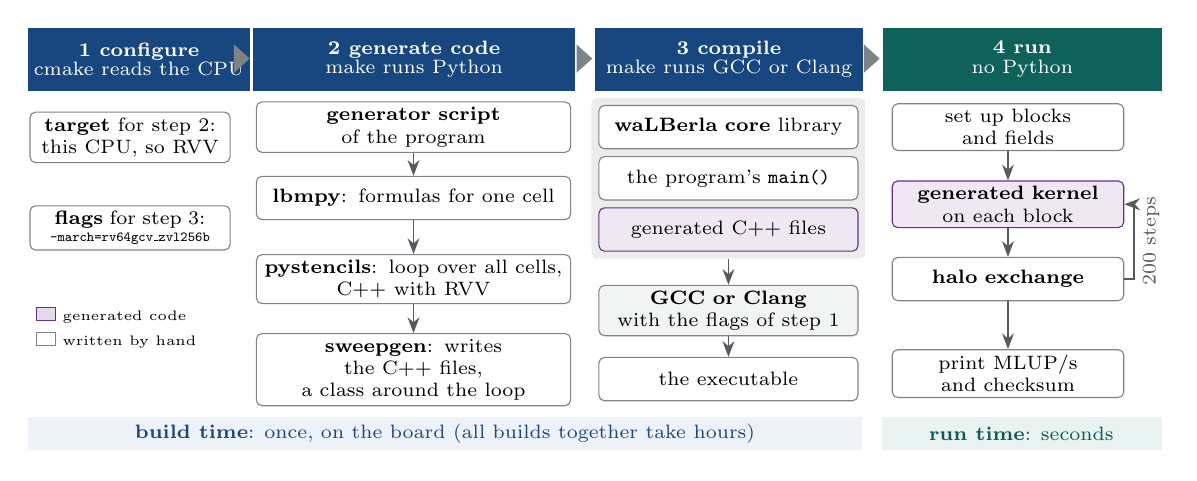
\begin{tikzpicture}[
    hdr/.style={font=\scriptsize\bfseries,text=white,align=center,inner sep=2pt,
      minimum height=8mm,anchor=north west},
    b/.style={box,font=\scriptsize,minimum height=5.5mm,inner sep=2pt,
      execute at begin node={\hyphenpenalty=10000\exhyphenpenalty=10000}},
    gen/.style={b,fill=psviolet!12,draw=psviolet!80!black},
    hdrarr/.style={fill=psgray!80},
    mk/.style={circle,text=white,font=\tiny\bfseries,inner sep=0pt,minimum size=3.7mm}]
  \ifbrmarkers\tikzset{mkl/.style={align=left}}\else\tikzset{mkl/.style={}}\fi
  % ---- column headers, with arrows from step to step --------------------------------
  \node[hdr,fill=psblue!75!black,minimum width=2.6cm] at (0,0)
    {1 configure\\[-1pt]{\mdseries cmake reads the CPU}};
  \node[hdr,fill=psblue!75!black,minimum width=4.1cm] at (2.85,0)
    {2 generate code\\[-1pt]{\mdseries make runs Python}};
  \node[hdr,fill=psblue!75!black,minimum width=3.4cm] at (7.2,0)
    {3 compile\\[-1pt]{\mdseries make runs GCC or Clang}};
  \node[hdr,fill=psteal!80!black,minimum width=3.55cm] at (10.85,0)
    {4 run\\[-1pt]{\mdseries no Python}};
  \foreach \x in {2.62,6.97,10.62}
    \fill[hdrarr] (\x,-0.22) -- ++(0.2,-0.18) -- ++(-0.2,-0.18) -- cycle;

  % ---- 1 configure: two settings for the later steps --------------------------------
  \node[b,text width=2.4cm] (a3) at (1.3,-1.4) {\textbf{target} for step 2:\\this CPU, so RVV};
  \node[b,text width=2.4cm,font=\tiny] (a2) at (1.3,-2.55)
    {{\scriptsize\textbf{flags} for step 3:}\\\code{-march=rv64gcv\_zvl256b}};
  \node[anchor=north west,font=\tiny,align=left,inner sep=0pt] at (0.1,-3.55)
    {\tikz\fill[psviolet!20,draw=psviolet!80!black] (0,0) rectangle (2.4mm,1.6mm);\ generated code\\[3pt]
     \tikz\draw[psgray!80] (0,0) rectangle (2.4mm,1.6mm);\ written by hand};

  % ---- 2 generate: the Python tool chain ---------------------------------------------
  \node[b,text width=3.85cm] (g0) at (4.9,-1.27) {\textbf{generator script} of the program};
  \node[b,text width=3.85cm] (g1) at (4.9,-2.17) {\textbf{lbmpy}: formulas for one cell};
  \node[b,text width=3.85cm] (g2) at (4.9,-3.2) {\textbf{pystencils}: loop over all cells,\\C++ with RVV};
  \node[b,text width=3.85cm] (g3) at (4.9,-4.35) {\textbf{sweepgen}: writes the C++ files,\\a class around the loop};
  \foreach \u/\v in {g0/g1,g1/g2,g2/g3} \draw[arr] (\u) -- (\v);

  % ---- 3 compile: hand-written and generated C++ together ----------------------------
  \node[b,mkl,text width=3.15cm] (i1) at (8.9,-1.27) {\textbf{waLBerla core} library};
  \node[b,mkl,text width=3.15cm] (i2) at (8.9,-1.92) {the program's \code{main()}};
  \node[gen,text width=3.15cm] (i0) at (8.9,-2.57) {generated C++ files};
  \begin{scope}[on background layer]
    \node[fill=psgray!12,rounded corners=2pt,inner sep=2.5pt,fit=(i1)(i2)(i0)] (src) {};
  \end{scope}
  \node[b,text width=3.15cm,fill=psgray!8] (cc) at (8.9,-3.6) {\textbf{GCC or Clang}\\with the flags of step 1};
  \node[b,text width=3.15cm] (exe) at (8.9,-4.47) {the executable};
  \draw[arr] (src) -- (cc);
  \draw[arr] (cc) -- (exe);

  % ---- 4 run: set up, then the time loop ---------------------------------------------
  \node[b,text width=2.8cm] (r0) at (12.45,-1.27) {set up blocks and fields};
  \node[gen,text width=2.8cm] (r1) at (12.45,-2.25) {\textbf{generated kernel}\\on each block};
  \node[b,text width=2.8cm] (r2) at (12.45,-3.2) {\textbf{halo exchange}};
  \node[b,text width=2.8cm] (r3) at (12.45,-4.4) {print MLUP/s and checksum};
  \draw[arr] (r0) -- (r1);
  \draw[arr] (r1) -- (r2);
  \draw[arr] (r2.east) -- ++(0.12,0) |- (r1.east);
  \node[lbl,rotate=90] at (14.27,-2.72) {200 steps};
  \draw[arr] (r2) -- (r3);

  % ---- time bands ----------------------------------------------------------------------
  \fill[psblue!8] (0,-4.95) rectangle (10.6,-5.37);
  \node[font=\scriptsize,text=psblue!75!black] at (5.3,-5.16)
    {\textbf{build time}: once, on the board (all builds together take hours)};
  \fill[psteal!10] (10.85,-4.95) rectangle (14.4,-5.37);
  \node[font=\scriptsize,text=psteal!75!black] at (12.62,-5.16) {\textbf{run time}: seconds};

  % ---- markers: what we changed ------------------------------------------------------
  \ifbrmarkers
    \tikzset{mk/.append style={minimum size=3.2mm}}
    %   \brmark: on top of the box's upper border; \brmarkin: inside the box, at its right end
    \def\brmark#1#2#3#4{% node, slot (0 = rightmost), colour, number
      \node[mk,fill=#3] at ([xshift={-2.2mm-#2*3.6mm},yshift=1.3mm]#1.north east) {#4};}
    \def\brmarkin#1#2#3#4{%
      \node[mk,fill=#3] at ([xshift={-2.2mm-#2*3.6mm}]#1.east) {#4};}
    \brmark{a2}{0}{psblue}{1}   \brmark{a2}{1}{psteal}{8}
    \brmark{g0}{0}{psblue}{3}
    \brmark{g2}{0}{psblue}{2}   \brmark{g2}{1}{psteal}{5}   \brmark{g2}{2}{psteal}{12}
    \brmark{g3}{0}{psteal}{6}   \brmark{g3}{1}{psteal}{10}
    \brmarkin{i1}{0}{psteal}{11} \brmarkin{i1}{1}{psteal}{7}
    \brmarkin{i2}{0}{psteal}{9}    \brmarkin{i2}{1}{psblue}{3}
    \brmark{cc}{0}{psblue}{4}
  \fi
\end{tikzpicture}
}}

  \vspace{1.5mm}
  {\scriptsize\renewcommand{\arraystretch}{0.95}
  \begin{tabular}{@{}lll@{}}
    \tagdot{psblue}\ \textbf{part 1: make it work} & \tagdot{psteal}\ \textbf{part 2: make it fast}
      & \tagdot{psteal}\ \textbf{part 2: the last three changes}\\
    1 RISC-V compiler flags & 5 prefetch, instruction choice, row addresses & 10 no density and velocity output\\
    2 RVV target in pystencils & 6 in-place kernels \quad 7 their halo exchange & 11 halo copy per direction\\
    3 benchmark program \quad 4 Clang fix & 8 X60 flag for Clang \quad 9 in-place time loop & 12 split kernel\\
  \end{tabular}\par}
\end{frame}

\end{document}
